%------------------ PA_DerCoachingBot_Wellenhofer_Max_28464.tex ------------------------------------------------
%
% Ausarbeitung zum Modul Projektstudium 
% im Fernstudium der Informatik an der Hochschule Trier 
% 
% Author: Maximilian Wellenhofer
% Betreuer: Prof. Dr. Georg Schneider
%
% Wintersemester 2021/22
%
%-------------------------------------------------------------------------------


%------------------ Präambel ---------------------------------------------------
\documentclass[envcountsame, envcountchap, deutsch]{i-studis} % scrartcl?

\usepackage[utf8]{inputenc}

\usepackage[a4paper]{geometry}
\usepackage[english, ngerman]{babel}

\usepackage[pdftex]{graphicx}
\usepackage{epstopdf}

\usepackage{listings}

\usepackage[german, ruled, vlined]{algorithm2e}
\usepackage{amssymb, amsfonts, amstext, amsmath}
\usepackage{array}
\usepackage[skip=10pt]{caption}
\usepackage[usenames, dvipsnames]{color}
\usepackage[pdftex, plainpages=false]{hyperref}
\usepackage{textcomp}

\usepackage{minted} % python interpreter
\usemintedstyle{manni}%{vs}%{pastie}%{autumn}%{emacs}%{tango}%{rrt}%{manni}

\usepackage{bibgerm}
\bibliographystyle{geralpha}

\usepackage{makeidx}
\usepackage{multicol}
\makeindex

\pagestyle{myheadings}
\setlength{\textheight}{1.1\textheight}

\lstset{
	basicstyle=\scriptsize\ttfamily,
	commentstyle=\scriptsize\ttfamily\color{Gray},
	identifierstyle=\scriptsize\ttfamily,
	keywordstyle=\scriptsize\ttfamily,
	stringstyle=\scriptsize\ttfamily,
	tabsize=4,
	numbers=left,
	numberstyle=\tiny,
	numberblanklines=false,
	frame=single,
	framesep=3mm,
	framexleftmargin=7mm,
	xleftmargin=10mm,
	linewidth=144mm,
	captionpos=b,
}


%------------------ Manuelle Silbentrennung ------------------------------------
\hyphenation{Ele-men-tar-ob-jek-te ab-ge-tas-tet Aus-wer-tung House-holder-Matrix Least-Squares-Al-go-ri-th-men}


%------------------ Titelseite -------------------------------------------------
\begin{document}

\title{Der Coaching Bot}
\subtitle{The Coaching Bot}

\author{Maximilian Wellenhofer}

\supervisor{Prof. Dr. Georg Schneider}

\address{Zürich}
\submitdate{28.03.2022}

%------------------ Projektart -------------------------------------------------
%\project{Bachelor-Projektarbeit}
%\project{Bachelor-Abschlussarbeit}
\project{Master-Projektstudium}
%\project{Master-Abschlussarbeit}
%\project{Seminar}
%\project{Hausarbeit}

\mytitlepage

%------------------ Vorwort, Kurzfassung, Verzeichnisse ------------------------
\frontmatter
%\preface

Ein Vorwort ist nicht unbedingt nötig. Falls Sie ein Vorwort schreiben, so ist dies der Platz, um z.B. die Firma vorzustellen, in der diese Arbeit entstanden ist, oder um den Personen zu danken, die in irgendeiner Form positiv zur Entstehung dieser Arbeit beigetragen haben.

Auf keinen Fall sollten Sie im Vorwort die Aufgabenstellung näher erläutern oder vertieft auf technische Sachverhalte eingehen.
								% Vorwort (optional)
\kurzfassung

\paragraph{Provisionierung eines Bots, der die OnBoarding-Phase eines Coaching Programms automatisiert.}




In der Kurzfassung soll in kurzer und prägnanter Weise der wesentliche Inhalt der Arbeit beschrieben werden. Dazu zählen vor allem eine kurze Aufgabenbeschreibung, der Lösungsansatz sowie die wesentlichen Ergebnisse der Arbeit. Ein häufiger Fehler für die Kurzfassung ist, dass lediglich die Aufgabenbeschreibung (d.h. das Problem) in Kurzform vorgelegt wird. Die Kurzfassung soll aber die gesamte Arbeit widerspiegeln. Deshalb sind vor allem die erzielten Ergebnisse darzustellen. Die Kurzfassung soll etwa eine halbe bis ganze DIN-A4-Seite umfassen.

Hinweis: Schreiben Sie die Kurzfassung am Ende der Arbeit, denn eventuell ist Ihnen beim Schreiben erst vollends klar geworden, was das Wesentliche der Arbeit ist bzw. welche Schwerpunkte Sie bei der Arbeit gesetzt haben. Andernfalls laufen Sie Gefahr, dass die Kurzfassung nicht zum Rest der Arbeit passt.

\kurzfassungEN

The same in English.
							% Kurzfassung/Abstract
\tableofcontents										% Inhaltsverzeichnis
\listoffigures											% Abbildungsverzeichnis (optional)
\listoftables											% Tabellenverzeichnis (optional)
\lstlistoflistings										% Listings (optional)


%------------------ Kapitel ----------------------------------------------------
\mainmatter
\chapter{Einleitung und Problemstellung} \label{Einleitung und Problemstellung}
        
    Viele junge Menschen die nach einem abgeschlossenen Studium in die Arbeitswelt einsteigen, haben keine oder wenig Erfahrung damit, wie sie sich vorbereiten sollen oder welche Schritte erforderlich sind, um einen erfolgreichen Start zu schaffen. Persönliche Beratungsleistungen und speziell Einzel-Coaching können dabei helfen, sich effektiv vorzubereiten und einen erheblichen Wettbewerbsvorteil bieten, sind aber für Berufseinsteiger ohne signifikante finanzielle Mittel meist weder zugänglich noch erschwinglich. Auch Professionals mit hinreichenden Mitteln haben oft Hemmungen und die Einstiegshürde für eine erste Session ist hoch. Diese Hürde soll für beide Zielgruppen herabgesetzt werden. Für eine unkomplizierte und intuitive Ansprache gewinnen digitale, mobile Messenger-Dienste und Social-Media-Kanäle zunehmend an Relevanz. Interaktionen mit jungen Absolventen auf klassischen Websiten stellen sich erfahrungsgemäß vor Allem im persönlichen Networking als wenig erfolgreich heraus.\\
    \\
    Darüber hinaus geht man als Coach mit einem Erstgespräch immer in Vorleistung, weil die erste Kennenlern-Session meist gratis angeboten werden muss, um überhaupt Neukunden zu gewinnen. 
    Aus dem Bedürfnis heraus, mit geringem kontinuierlichen Planungs- und Koordinationsaufwand ein breit gefächertes Klientel im Coaching-Bereich aufzubauen, sollen diverse Kanäle geprüft werden. Ziel ist es, Systeme und Technologien für einen standardisierten Onboarding-Mechanismus und einen entsprechenden Workflow zu finden, um den Prozess bis zum Kennenlernen von manuellem Aufwand soweit als sinnvoll zu abstrahieren und damit verbundene Kosten auf ein Minimum zu reduzieren. Der Standardisierungscharakter ist deshalb sinnvoll, weil eine erste Kontaktaufnahme und Vorbereitung auf eine erste Sitzung erfahrungsgemäß sehr kongruent zueinander oder gar einem Skript folgend verlaufen. \\
    \\
    Coaching ist ein sehr persönliches Geschäftsfeld, in dem ein Web-Formular evtl. nicht den Konversations-Charakter aufweist, den man sich als Nutzer wünscht. Es entsteht eher der Eindruck einer Anmeldung für ein Programm. Ein Coaching ist aber eine Partnerschaft zwischen zwei Individuen. Die Erweiterung der Kommunikationskanäle um einen Chat-Bot wird das Problem nicht abschließend lösen, aber die Hypothese lautet, dass die Hemmschwelle gesenkt werden und höhere Conversions erreicht werden könnten. Die Abwendung vom Web-Browser als Kommunikationsmedium ist keine Neuerung der letzten Jahre und schreitet mit der steten Optimierung von Messenger-Diensten wie WhatsApp, Signal, Telegram und Kommunikationsoptionen via Social-Media-Portalen wie Instagram, Facebook, TikTok, SnapChat, etc. weiter voran. Ein Nebeneinander von Web-Formular und Chat-Bot kann helfen, die Conversion Rate für eine Dienstleistung auf ein neues Niveau zu heben. \cite{conversion} Es soll daher ein Proof of Concept für einen Chat-Bot entwickelt werden.\\ 
    \\ 
    \paragraph{Im Fokus stehen:}
    \begin{enumerate}
        \item Ein Nutzer kann einen Termin mit einem Dienstleister ohne dessen Zutun vereinbaren.
        \item Dem Dienstleister soll die repetitive, manuelle Akquise durch einen geführten, technisch gestützen, Ablauf erleichtert werden. 
        \item Es soll eine Alternative für den Kanal Web-Formular geboten werden. 
        \item Der Kanal soll einen kommunikativen Charakter aufweisen. (wie ein Chat-Bot)
        \item Das System soll durch Anbieter von Coaching-Dienstleistungen mit wenigen Vorkenntnissen leicht adaptierbar sein.
    \end{enumerate}
    
    Ziel des Projekts ist es also, eine erste Version des Coaching Bots zu programmieren, die es ermöglicht, persönliche Angaben zu machen und den Nutzer zu einer Terminvereinbarung hinzuführen. Um den Entwicklungsaufwand so gering wie möglich zu halten, wurde hierzu eine Reihe an Systemen analysiert. Eine detaillierte Aufschlüsselung der Systeme folgt in \ref{Verwandte Arbeiten} Verwandte Arbeiten und \ref{Grundlagen} Grundlagen.





\chapter{Verwandte Arbeiten}

    Ziel der Recherche war es, einen kleinen, selbst wartbaren open source Chatbot zu finden, der von angehenden Coaches mit minimalen Kenntnissen und einer einfach verständlichen Dokumentation ohne monetäre Mittel auf die eigenen Bedürfnisse angepasst, an einem beliebigen Ort gehostet und eine einfache, geskriptete OnBoarding-Phase durchlaufen kann. Analysiert man den Hintergrund der meisten Bots, so wird schnell klar: Die meisten Fraeworks sind zu mächtig, bieten zu umfangreiche und komplexe Feature-Sets, die für Enterprise-Grade-Software bestens geeignet sind, aber für die in der Problemstellung beschriebenen Zwecke zu weitreichend sind. Daneben sind ansonsten valable Optionen teilweise nicht direkt, aber in zweiter Instanz zu eng mit zu bezahlenden Systemen verknüpft, als dass diese ohne Weiteres genutzt werden könnten. Nach umfangreicher Recherche hat man sich ergo dazu entschieden, die Anforderungen selbst auf Basis der in \ref{Grundlagen} aufgeschlüsselten Systeme zu erfüllen. \\

    Analysierte Frameworks:
    \begin{enumerate}
        \item Microsoft Bot Framework
        \item Botkit
        \item Botpress
        \item Rasa
        \item Wit.ai
        \item OpenDialog
        \item Botonic
        \item Claudia Bot Builder
        \item Tock
        \item BotMan
        \item Bottender
        \item DeepPavlov
        \item Golem
        \item ParlAI by Facebook AI
        \item Ana
        \item Bot Libre
    \end{enumerate}


\section{Microsoft Bot Framework} \url{https://github.com/microsoft/botframework-sdk}
Als Corporate ist eine Nutzung des von Microsoft bereitgestellten Frameworks sicher aufgrund vielerlei Plug-and-play-Integrationen sinnvoll. Allerdings bindet man sich damit an die mit Kosten verbundene Cloud Plattform Azure. Das Open Source Kriterium ist also nicht erfüllt. 

\section{Botkit} \url{https://github.com/howdyai/botkit-cms}
Botkit ist im Microsoft Bot Framework aufgegangen. 

\section{Botpress} \url{https://botpress.com/}
Botpress ist ein sehr mächtiges Bot Framework, das grundsätzlich den oben genannten Anforderungen entspricht. Schnell wird aber klar, dass man als Laie umfangreiche Einarbeitung benötigt und, dass das Natural Language Understanding, das für fortgeschrittene Chatbos eines der Hauptfeatures ist, die hier geforderten Zwecke weit übersteigt.

\section{Rasa} \url{https://github.com/RasaHQ/rasa}
Rasa bietet mit seinem Story-Feature genau das, was man sich als Coach wünscht. Nämlich, den potenziellen Coachee mit auf seine persönliche Reise zu nehmen. Allerdings bedarf Rasa, um gut zu funktionieren eines umfangreichen Datensatzes, anhand dessen die AI lernen kann und das liegt uns leider nicht vor.

\section{Wit.ai} \url{https://github.com/wit-ai}
Wit.ai gehört Facebook (inzwischen Meta) und entspricht damit nicht unserer Vorstellung von freier Software.

\section{OpenDialog} \url{https://www.opendialog.ai/}
Open Dialog ist zwar open source, die Nutzung ist aber mit Lizenzgebühren verbunden.

\section{Botonic} \url{https://github.com/hubtype/botonic}
Botonic bietet genau das, was wir gesucht haben: Eine Kombination aus Text- und grafischen Schnittstellen. Allerdings sind wie auch für die Nutzung von Botonic, wie für Botpress, umfangreiche Vorkenntnisse erforderlich. Eine Weiterverwendung und Individualisierung durch weitere Coaches ist daher unwahrscheinlich.

\section{Claudia Bot Builder} \url{https://github.com/claudiajs/claudia-bot-builder}
Claudia Bot Builder reduziert die Komplexität, einen Bot selbst zu bauen und zu konfigurieren erheblich und bietet somit genau die Features, die eine einfache Adaption ermöglichen. Leider ist die Software aber ausschließlich auf AWS Lambda ausführbar und somit mit regelmäßigen Kosten verbunden. 

\section{Tock} \url{https://github.com/theopenconversationkit/tock}
Tock ist eine valable Stand Alone Lösung für Chat Bots. Allerdings ist die Kompatibilität mit Plattformen, die ausschließlich kommerziellen Corporationen gehören, nicht mit den Zielen des Coaching Bots vereinbar. 

\section{BotMan} \url{https://github.com/botman/botman}
Als das populärste Bot-Framework der Welt, stellt BotMan einen soliden Kandidaten für unseren Coaching Bot dar.

\section{Bottender} \url{https://github.com/yoctol/bottender}
Auch Bottender erfüllt auf den ersten Blick alle Anforderungen, die an das Framework gestellt wurden. Allerdings scheint es, als wären die Features, die für die Zwecke des Coaching-Bots benötigt werden, nicht einfacher zu implementieren als auf einer Chatbot Boiler Plate. Durch Bottender wären aber Komplexität und Gewicht der Applikation erheblich erhöht.

\section{DeepPavlov} \url{https://github.com/deepmipt/deeppavlov}
Das auf mächtige und qualitativ hochwertiges NLP ausgelegte Framework DeepPavlov ist weitaus zu mächtig und entspricht nicht dem geskripteten OnBoarding-Prozess, der für den CoachingBot verfolgt werden soll.

\section{Golem} \url{https://github.com/prihoda/golem}
Aus den gleichen Gründen wie bei Bottender und DeepPavlov ist uns auch Golem nicht dienlich. Weder werden für die erste Version des Bots NLU benötigt, noch bietet Golem mehr relevante Features, als die Vanilla-Version des Telegram-Bots.

\section{ParlAI by Facebook AI} \url{https://ai.facebook.com/blog/state-of-the-art-open-source-chatbot/}
Als Teil des Facebook- / Meta-Universums bietet ParlAI wahrscheinlich eines der besten NLPs, die aktuell verfügbar sind. Allerdings befindet sich das Framework noch in Produktion und das Feature wird nicht benötigt.

\section{Ana} \url{https://www.ana.chat/}
Ana bietet ein SDK, über das ein Chatbot in Applikationen integriert werden kann. Da wir aber bestehende Messenger Applikationen nutzen möchten, schließen wir Ana aus.

\section{Bot Libre} \url{https://www.botlibre.com/}
Bot Libre ist auf Android beschränkt. Ein dignifikanter Anteil aller Mobile-User wäre dadurch von unserer Zielgruppe ausgeschlossen.


\chapter{Grundlagen}

1. Python
2. Telegram API: 
3. SQL
4. PHP
5. HTML
6. Google Calendar API: 

API: https://googleapis.github.io/google-api-python-client/docs/dyn/calendar_v3.html 

Google Cloud Console: https://console.cloud.google.com/apis/credentials/consent?project=coaching-bot-339115 

Calendar API Python Quickstart Guide: https://developers.google.com/calendar/api/quickstart/python 

Verify own website: https://www.google.com/webmasters/verification/home?hl=en
\label{Konzept}
\chapter{Konzept}

\section{Grundkonzept}

	\begin{figure} %[hbtp]
		\centering
		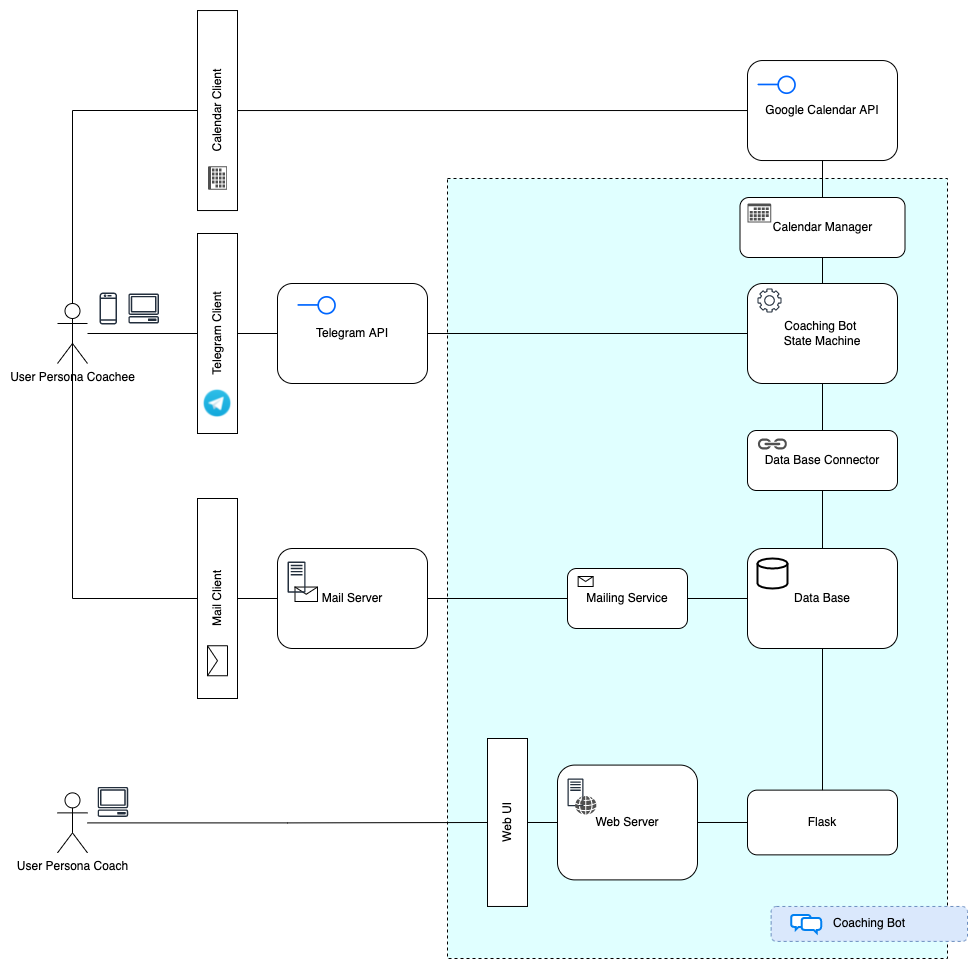
\includegraphics[width=1.0\textwidth]{images/220320_PA28464_Architecture.png}
		\caption{Konzeptionelle Architektur für das Projekt \emph{Der Coaching Bot}}
		\label{fig: architecture}
	\end{figure}

	Wie in Abbildung \ref{fig: architecture} skizziert, besteht der Kern des Bots auf einem endlichen Automaten (state machine), der Zustände vordefiniert und festlegt, wann sich welcher Nutzer in welchem Zustand befindet und von welchem in welchen Zustand er sich bewegen darf. An diesen Kern bindet sind als zentrales Steuerungselement des Bots alle anderen Systeme angebunden. Dazu gehören:
	\begin{enumerate}
		\item Die Datenbank zur Speicherung der Nutzerdaten
		\item Die Telegram API, über die die Kommunikation mit dem Telegram Client abgewickelt wird
		\item Die Google Calendar API, über die Events erstellt und versendet werden können
		\item Den Mail Server, über den E-Mails an den nutzer versendet werden können.
	\end{enumerate} 

	Der Nutzer interagiert mit dem ganzen System durch vier Kanäle - hier links ersichtlich:
	\begin{enumerate}
		\item Telegram Client: Kommunikation mit dem Bot
		\item Calendar Client: Erhalt, Annahme sowie Ablehnung der vereinbarten Termine
		\item Mail Client: Erhalten der Zusammenfassung und Bestätigung
		\item Web Browser: Übersicht über Anmeldungen und Terminkalender
	\end{enumerate}

	Der Bot wird von Benutzern (links oben) via einem der verfügbaren Telegram Clients angesprochen und reagiert auf die Eingabe entsprechend. So können verschieden Funktionen ausgelöst werden. Bspw. werden Antworten zurückgegeben, Informationen gespeichert oder es wird ein Vorschlag gemacht und an den Nutzer zurückgegeben. Der Bot soll mit mehreren Benutzern gleichzeitig sprechen können. Das wird ermöglicht, weil alle Reaktionen des Bots mit der Kennung des jeweiligen Nutzers verknüpft sind. So spricht der Bot den Nutzer mit Namen an oder kann sich daran erinnnern, welche Fragen schon beantwortet wurden und welche nicht. \\ \\

	Daneben gibt es einen zweite, sehr einfache Web-Applikation, die auf Flask basiert und eine Web-GUI zur Verfügung stellt, über die die gesammelten Informationen dargestellt werden können. So kann ein Coach (links unten) sich, nachdem Bewerber den Prozess beendet haben, alle gesammelten Informationen sowie vereinbarte Termine in einer einfachen Web-GUI ansehen.

\section{Zustände \& Konversationsfluss}

	Im folgenden Zustandsdiagramm ist der Konversationsfluss des Bots auf hohem Abstraktionsniveau, nämlich als endlicher Automat (state machine) abgebildet. Es wird deutlich, dass der Bot einem einfachen Skript folgt und komplizierte Loops vermieden werden. 
	\begin{figure} %[hbtp]
		\centering
		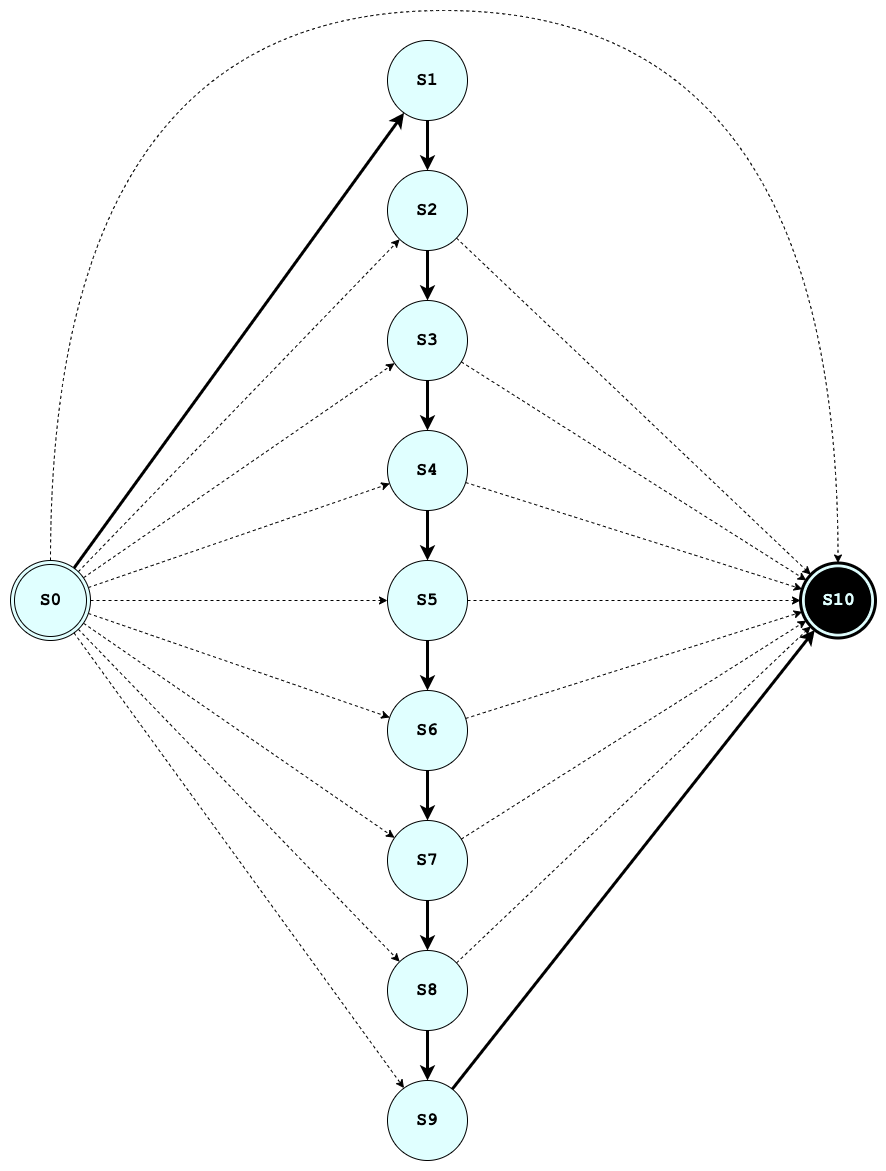
\includegraphics[width=1.0\textwidth]{images/220320_PA28464_State-Machine.png}
		\caption{Endlicher Automat des Konversationsflusses des Bots}
		\label{fig: state machine}
	\end{figure}

	Zustände:
	\begin{table} %[hbtp]
		\centering
		\begin{tabular}{l | l l l l}
			\textbf{Zustände} 	& \textbf{Beschreibung}\\
			\hline
			S0 					&		 START 			&		 Start: Applikation gestartet\\
			S1 					&		 BIO 			&		 Eingabemöglichkeit Biographie\\
			S2 					&		 GENDER 		&		 Eingabemöglichkeit Geschlecht\\
			S3 					&		 BIRTHDATE 		&		 Eingabemöglichkeit Geburtsdatum\\
			S4 					&		 EMAIL 			&		 Eingabemöglichkeit E-Mail Adresse\\
			S5 					&		 TELEPHONE 		&		 Eingabemöglichkeit Telefonnummer\\
			S6 					&		 LOCATION 		&		 Eingabemöglichkeit Ort\\
			S7 					&		 PHOTO 			&		 Eingabemöglichkeit Bild\\
			S8 					&		 SUMMARY 		&		 Zusammenfassung Daten\\
			S9 					&		 APPOINTMENT	&		 Terminvereinbarung \\
			S10 				&		 ENDE 			&		 Ende: Applikation beendet\\

		\end{tabular}
		\caption{Zustände des Konversationsflusses}
		\label{tab: states}
	\end{table}

	Der Haupt-Pfad ist hier fett eingezeichnet. Nebem diesem ist es aber auch möglich, dass der Nutzer nach einiger Zeit zum Bot zurück kommt und gerne an der Stelle weitermachen würde, wo er aufgehört hat. In diesem Fall, dient der Zustand \verb|S0| (START) als zentraler Einstiegspunkt. Hier wird analysiert, ob der Nutzer schon bekannt ist und falls ja, bis wohin er den Prozess bereits durchlaufen hat. Dann wird er dorthin weitergeleitet. Daher ist es möglich von START zu allen anderen Zuständen zu kommen, auch wenn das nicht die Regel ist. Hat der Nutzer den Prozess bereits abgeschlossen, so kann er sogar von S0 direkt in S10 landen und wird entsprechend benachrichtigt. Da dem Nutzer die Möglichkeit gegeben werden soll, den Prozess jederzeit zu beenden, ist es auch möglich, von jedem Zustand in \verb|S10| zu gelangen. \footnote{Der Konversationsfluss ist in einer sehr detaillierteren Ansicht verfügbar, in der der Unterschied zwischen dem hohen Abstraktionsniveau des Automaten und der Realität sichtbar wird. So lässt sich leicht erkennen, wo die Konversation beginnt und welche Zustände und Übergänge möglich sind: \url{girthub}} 
\label{Realisierung}
\chapter{Realisierung}

    \section{Realisierung User Journey}

    Die in Abschnitt \ref{User Journey} beschriebene User Journey soll folgendermaßen umgesetzt werden:

    \begin{enumerate}
        \item Sobald der User eine Verbindung zum Bot herstellt, wird seine Telegram-ID geloggt.
        \item Da Nutzer derlei Angaben zeitlich sehr volatil und nicht am Stück vornehmen, muss der Nutzer jederzeit die Möglichkeit haben, den Chat zu verlassen und zu ihm zurückkehren\footnote{Daher die Erfordernis der Bindung aller Informationen an die User-ID} und die Kommunikation mit dem Bot wiederaufzunehmen.
        \item Informationen, die der User eingibt, werden mit der Telegram-ID des Users verknüpft und i.e. via einem SQL-python-connector in eine ausgelagerte DB (i.e. mySQL oder SQLight) geschrieben.
        \item Damit getrackt werden kann, welche Fragen der User schon beantwortet hat, muss es eine Funktion geben, die nach jeder Benutzereingabe abfragt, welche Fragen schon beantwortet sind. Dies kann entweder über einen Cache passieren oder über eine DB-Abfrage. Via Ausschluss bekommt man dann die noch offenen Fragen und kann diese an einer passenden Stelle in der Journey oder auf Befehl an den User zurückspielen.
        \item Genau dann, wenn diese Liste ausgegeben wird, soll der User wählen können, mit welcher Fragen er fortfahren möchte. Das könnte über ein custom Keyboard passieren.
        \item Damit das alles funktioniert muss der Bot immer wissen, mit welchem User er gerade kommuniziert und welche Frage gerade beantwortet wird. (evtl. Sessions - tbd)
        \item Sowohl Coach als auch Coachee sollen zu jeder Zeit (ab Vollendung von Stufe 1) die Möglichkeit haben, eingegebene Daten einzusehen.
        \begin{enumerate}
            \item Telegram-ID
            \item Gender
            \item First Name
            \item Last Name
            \item E-Mail-Adresse
            \item Telefonnummer
            \item Picture
            \item Biography
            \item Problems
            \item Desired Position
            \item Initial Questions
            \item evtl. Weitere
        \end{enumerate} 
        \item Der Coachee kann seine Daten vom Bot abfragen. >> /summary Diese sollen nach Möglichkeit etwas aufbereitet werden. (tbd)
        \item Für den Coach soll eine Übersicht über alle Coachees in Form einer Web-GUI gebaut werden, die diese Informationen unkompliziert darstellt.
        \item Sobald alle Informationen eingereicht sind, soll zur Terminvereinbarung ein Datepicker eingebunden und angezeigt werden, der im Hintergrund einen google calendar managed. Datum und Zeit können ausgewählt werden. Die Standard-Zeit beträgt 1h und es können nur Termine ausgewählt werden, die noch nicht belegt sind. (Auf die Auswahl der Zeitzone wird hier verzichtet, da das Coaching-Angebot aktuell nur in CET angeboten wird.)
        \item Der Benutzer bekommt eine schriftliche Bestätigung in Form einer E-Mail mit seinen Daten und dem vereinbarten Termin.
        \item Der Coach bekommt eine E-Mail mit den Infos zum neuen Bewerber und einem Link zur Übersicht.
        \item Der Bot verabschiedet sich. (Ende der Konversation)

    \end{enumerate}



    \section{Telegram Bot Framwork}

        \subsection{Generierung Telegram Bot} \label{botfather}

            Als ersten Schritt zur Erschaffung eines Telegram-Bots wird der Bot-Father\footnote{\url{https://core.telegram.org/bots\#6-botfather}} konsultiert.  Er erstellt das Framework, registriert den Bot und gibt ein API-Token zurück, das verwendet werden kann, um sich gegenüber der Telegram-Bot-API als Entwickler zu identifizieren. \cite{telegramAPI} Das Token dient als einzige Identifikationsmethode. Jeder, der in Besitz des Schlüssel ist, kann den zugehörigen Bot theoretisch nutzen und bearbeiten. Das Token ist also an einem sicheren Ort aufzubewahren und nicht in einer öffentlichen Versionierung freizugeben.

        \subsection{Vanilla Bot Implementierung}
            Als Basis (boiler plate) für den Coaching Bot (fortan \glqq Bot\grqq) nutzen wir die breit in der Community abgestütze Implementierung \textbf{Conversation Bot} \cite{conversationBot}. Sie stellt uns die basale Anbindung an die State Machine zur Verfügung und ist einfach genug, um als Einstieg in einen vordefinierten Bot zu fungieren. Im Gegensatz dazu ist der \glqq Nested Converation Bot\grqq  schon zu umfangreich und zu mächtig für unsere Zwecke.

            Die Kommunikationslogik des Bots basiert auf einer State Machine. Die Zustände, in denen der Bot sich befinden kann, sind vordefiniert und immer mit einer Aktion und einer Reaktion verbunden. Aktionen werden meist von Seiten des Benutzers durch eine Eingabe oder einen Befehl ausgelöst. Reaktionen sind in Funktionen vordefiniert. Deren Umfang wird im Folgenden funktional und in \ref{Implementierung} Implementierung technisch beschrieben.

    
    \section{Meta-Funktionen}
        Neben den Hauptfunktionen des Bots (Funktionen, die zum Gesprächsfluss gehören), gibt es eine Reihe an Meta-Funktionen, die dem Nutzer zur Verfügung stehen, um eine Konversation zu starten, zu beenden, persönliche Daten zu löschen oder die Hilfe auszugeben.

        \subsection{Start: Eine Konversation beginnen}
            Der Bot kann gestartet werden (Aktion) und gibt eine Begrüßungsnachricht zurück. Gleichzeitig erfasst er grundsätzliche Informationen des Nutzers und schreibt diese in eine Datenbank. Aber diesem Zeitpunkt, kennt die Applikation den Benutzer und kann weitere Informationen über ihn speichern oder individuell auf Eingaben reagieren.
            Eine der großen Herausforderungen für den Bot besteht darin, einen Nutzer wiederzuerkennen und ihn am richtigen Punkt zurück in den Konversationsfluss zu platzieren. Diese Erfahrung soll für den Nutzer nicht angestrengt wirken, sondern so, als würde der Bot ihn schon kennen und einfach da weitermachen, wo man aufgehört hat. Die technische Komplexität besteht darin, dass das Feature besonders dann funktionieren soll, wenn der Bot neu gestartet wurde. Diese Memory-Funktion muss am Beginn der Konversation stattfinden.

        \subsection{Ende: Konversation manuell beenden}
            Hat der Nutzer eine Konversation gestartet, so kann er diese auch wieder beenden. Die Konversation muss nicht zuende geführt worden sein. Über einen kurzen Befehl \verb|/cancel| wird der Bot beendet und personenbezogene Daten werden aus der Datenbank gelöscht. Dabei ist darauf zu achten, dass der Nutzer nur seine eigenen Daten löschen kann. Hat der Nutzer seine Konversation bereits beendet, so ist \verb|/cancel| nicht mehr verfügbar. Möchte der Nutzer seine Daten dennoch löschen, so steht ihm stattdessen der Befehl \verb|/delete| zur Verfügung.

        \subsection{Persönliche Daten löschen}
            Zu jeder Zeit hat der Nutzer die Möglichkeit, die eigenen Daten via dem Befehl \verb|/delete| zu löschen. Die Funktion ist mit einem \glqq Reset-Knopf\grqq  zu vergleichen. Das Resultat ist nämlich, dass der Bot den Benutzer nicht mehr kennt. Er weiß nicht, dass er schon einmal da war und auch nicht, welche Angaben er gemacht hat oder nicht. So kann man den Bot nach fehlerhafter Eingabe oder, falls man neu anfangen möchte, einfach zurücksetzen.

        \subsection{Hilfe-Funktion aufrufen}
            Die Hilfe-Funktion gibt eine Beschreibung der Interaktionen-Optionen aus, die es gegeneüber dem Bot gibt. So werden alle Befehle einfach erklärt und können auch direkt aus der Hilfe heraus aufgerufen werden. 

        \subsection{Überspringen}
            Die meisten Zustände des Bots erlauben es dem Benutzer, die aktuelle Frage zu überspringen. Vor allem, wenn es um personenbezogene oder private Informationen geht, die der Nutzer preisgibt, ist der Befehl \verb|/skip| verfügbar. Für jeden Zustand, in dem \verb|/skip| verfügbar ist, ist eine individuelle Reaktion auf das Überspringen vorgesehen, die den Nutzer trotzdem abholt um in den nächsten Zustand leitet. Die einzelnen Übersprunkgsfunktionen werden in \ref{Implementierung} Implementierung genauer erklärt.

    \section{Hauptfunktionen}

        \subsection{Abfragen des Geburtsdatums}    
            Um zu erfahren, wie alt der Bewerber ist, möchten wir das Geburtsdatum abfragen. Dabei ist wichtig, dass das Datum in einem sinnvollen Format eingegeben wird. (Siehe Eingabe-Validierung.)

        \subsection{Hintergrund des Nutzers}
            Für eine Coaching-Session ist es besonders wichtig, den Coachee besser kennenzulernen. Zu diesem Zweck hat der Nutzer die Möglichkeit, etwas über sich zu erzählen. Erwartet wird hier kein komplettes Motivationsschreiben, sondern einfache, kurz formulierte Beweggründe dafür, dass man gerne mit dem Personal Coaching beginnen möchte. 
        
        \subsection{Abfragen des Geschlechts des Nutzers}
            Um den Nutzer in der Folegkommunikation korrekt anzusprechen, wird nach dem Geschlecht des Nutzers gefragt. Neben der Option, die Frage überspringen zu können, präsentiert der Bot den Nutzer mit mehr als 2 Optionen, um diversen Geschlechtern gerecht zu werden.
        
        \subsection{Abfragen der E-Mail Adresse des Nutzers}
            Um dem Nutzer eine E-Mail mit allen erfassten Daten zusenden zu können und dem eigentlichen Zweck des Bots nachzukommen - einen Termin vereinbaren zu können - benötigt der Bot eine valide E-Mail-Adresse des Nutzers. Um die Wahrscheinlichkeit zu erhöhen, dass bei dieser Eigabe keine Fehler passieren, ist auch hier eine Eingabe-Validierung hinterlegt.
        
        \subsection{Abfragen der Telefonnummer des Nutzers}
            Am Ende des Konversationsflusses hat der Nutzer die Möglichkeit, einen ersten Termin zu vereinbaren. Dabei handelt es sich um einen unverbindlichen Telefontermin. Um den Nutzer zu einer festgelegten Zeit erreichen zu können, wird hier die Telefonnummer des Nutzers erfasst. Da der Service aktuell nur in der DACH-Region angeboten wird, können hier nur Telefonnummern mit der Länderkennung Deutschland, Österreich und der Schweiz angegeben werden. 
        
        \subsection{Abfragen des Standorts des Nutzers}
            Der Coaching-Service soll primär und vorerst nur in der DACH-Region angeboten werden. Daher soll der Standort des Nutzers abgefragt werden. Eine Geo-Fencing-Funktion würde für unseren Zweck hier zu weit gehen, weil wir auch Personen die Chance geben wollen, sich für den Dienst anzumelden, die aktuell im Ausland sind. So bietet die Telegram-App dem Nutzer die Möglichkeit, den Ort, den er teilen möchte, spotan selbst auszuwählen.
        
        \subsection{Abfragen des Bilds des Nutzers}
        Informationen aller Nutzer werden als Resultat der Teilnahme am On-Boarding in einer Web-GUI ausgegeben. Hier wird neben den Informationen zum Bewerber auch ein Bild angezeigt. So kann der Coach sich besser auf ein erstes Treffen einstellen. 
        
        \subsection{Zusammenfassungs-Funktion}
            Ziel des Bots ist ein hohes Maß an Transparenz auf allen Seiten. Der Nutzer weiß nicht nur, dass seine Daten erfasst wurden, sondern am Ende des Konversationsflusses werden diese auch automatisch zurückkommuniziert. Dies passiert auf zweierlei Wegen. Neben einer Telegram-Nachricht wird dem Nutzer auch eine Zusammenfassung in Form einer E-Mail an die angegebene Adresse gesendet. Darüber hinaus hat der Nutzer die Möglichkeit, die Zusammenfassung jederzeit manuell abzurufen. So kann er jederzeit einsehen, welche Informationen bereits übergeben wurden und welche noch fehlen.

            
    \section{Support-Funktionen}
        
        \subsection{Eingabe-Validierung}
        Bei einigen Angaben ist es besonders wichtig, dass Eingaben auf korrekte Formate geprüft werden. So müssen bspw. E-Mail-Adresse sowie Telefonnummer des Nutzers stimmen, um weitere Funktionen des Bots zu nutzen. Um die Wahrscheinlichkeit dafür, dass diese Eingaben korrekt sind, zu steigern, werden ausgewählte Eingaben auf Formatfehler geprüft und der Nutzer bei falscher Eingabe um eine erneute Eingabe gebeten.
        
        \subsection{Konstruktion E-Mail}
        Die E-Mail, die am Ende des Konversationsflusses ausgegeben wird, wird separat aus verschiedenen Bausteinen zusammengesetzt. Dafür kommen Informationsabfragen gegen die Datenbank mit der Ansprache eines Mail-Servers zusammen.
        
    
    \section{Datenbank} \label{Realisierung Datenbank}
        Fast alle Informationen über den Nutzer werden in einer Datenbank gespeichert. Ausgenommen ist nur das Bild, das der Nutzer hochlädt. So können einzelne Werte jederzeit verwendet werden, um Nutzer-spezifische Reaktionen zu gestalten.
        Dem Nutzer stehen die meisten Datenbank-Operationen implizit und wenige explizit zur Verfügung. Daten werden implizit gespeichert und abgerufen. Explizit können Daten gelöscht werden. Zur Realisierung wird eine SLQlite Datenbank genutzt. Diese einfache Datenbank ist für den Zweck des Coaching-Bots vollkommen ausreichend. Weder ist mit immensen Nutzerzahlen, noch mit vielen gleichzeitigen Operationen oder einer riesigen Datemenge zu rechen, was für mächtigere Lösungen sprechen würde.
        Da keine komplexen berechnungen auf den Daten ausgeführt werden, sondern nur basale CRUD-Operaionen geplant sind, gibt es nur eine Tabelle (siehe Abb. \ref{fig: data base model}), in der alle Nutzerdaten gespeichert sind.
        \begin{figure} %[hbtp]
            \centering
            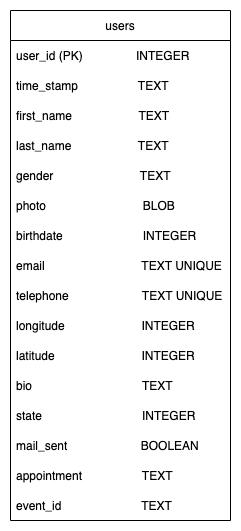
\includegraphics[width=0.5\textwidth]{images/220325_PA28464_DataBaseModel.png}
            \caption{coachingBot\_DB - Datenbankmodell}
            \label{fig: data base model}
        \end{figure}


    \section{Anbindung Datenbank an Python}
        Um eine individuelle Implementierung eines Database-Connectors zu vermeiden, bedient die Applikation sich der sqlite3-Bibliothek. Sie ermöglicht es, klassische Datenbank-Operationen direkt aus einem Python-Skript heraus anzustoßen und dient hier als Database-Connector. Die Operationen selbst werden in handelsüblichem SQL formuliert und übergeben.


    \section{Kalender}
        Um am Ende des Konversationsflusses einen ersten Termin mit einem Coach vereinbaren zu können, muss der Nutzer einen freien Termin auswählen können und für diesen eine Einladung beantragen. Zu diesem Zweck wurde die Google Calendar API angebunden. Der Nutzer wird zunächst gefragt, ob er überhaupt einen Termin vereinbaren möchte. Daraufhin wird die API abgefragt und dem Nutzer werden drei Termine vorgeschlagen. Mit einem Klick kann der gewünschte Termin dann ausgewählt werden. Kurz darauf erhält der Nutzer eine Termineinladung an die zuvor angegebene E-Mail-Adresse und kann diese im persönlichen Kalender-Client annehmen oder ablehnen. \\
        Eine Kennenlern-Sitzung dauert 50 Minuten. Vorschläge sollen über eine Spanne von 10 Tagen verteilt sein und nur an Wochentagen und zu Geschäftszeiten möglich sein. Da sich Geschäftszeiten ändern können und dazu keine Anpassung am Programmcode notwendig sein soll, werden Geschäftszeiten direkt im entsprechenden Kalender festgelegt.

    
    \section{Web-GUI}
        Um gesammelte Daten und vereinbarte Termine am Ende anzeigen zu können, wird eine einfach Web-GUI mittels HTML und CSS erstellt und auf einem lokalen Flask Web-Server deployed. Die Anbindung an die Datenbank ist bereits über den Database Connector implementiert, der auch für die Web-GUI die Daten liefert. Für eine einfache, direkte Einsicht in vereinbarte Termine, wird eine Google-Calendar View eingebunden. 
\label{Implementierung}
\chapter{Implementierung}

    Die im Kapitel \ref*{Realisierung} Realisierung erarbeiteten Ansätze wurden umgesetzt. Die Systeme und Ergebnisse werden im Folgenden beschrieben.

    \section{main.py - Anmeldung, Updater, Dispatcher und Handler-Konfiguration} \label{main.py}
        Auf diese Mechanismen der \verb|main.py|-Methode wird in den folgenden drei Code-Abschnitten eingegangen:
        \begin{lstlisting}[language=Python, caption={bot/main.py(1) - Authentifizierung und Schlüssel-Übergabe an den Updater}\label{code: bot/main.py 1}]
# Hand over API_TOKEN to the bot
bot = telegram.Bot(token=API_KEY)

def main() -> None:
# Creates the updater and passes the API_TOKEN to it.
updater = Updater(API_KEY)
        \end{lstlisting}
        Die \verb|main.py|-Methode basiert auf dem im Kapiel \ref*{Grundlagen} Grundlagen vorgestellten Conversation Bot. Sie importiert alle Handler, authentifiziert sich gegenüber der Telegram API (wie in Listing \ref*{code: bot/main.py 1} zu sehen), instanziiert den Bot und seinen Dispatcher und bindet dann in einem genesteten Aufbau Message- und Command-Handler and Conversation-Handler und diese wiederum an den Dispatcher, um den Bot in einen Zustand zu versetzen, in dem er Befehle entgegennehmen und entsprechend reagieren kann. \\
        
        Dispatcher liefern Nachrichten an den User aus. Pro Bot gibt es grundsätzlich mind. einen Dispatcher. Der Coaching Bot hat aber mehrere für mehrere Konversationsstränge. An den Dispatcher werden Conversation- sowie CommandHandler gebunden und konfiguriert (wie in Listing \ref*{code: bot/main.py 1} ersichtlich).\\
        Der Conversation-Handler bildet die in Abb. \ref*{fig: state machine} konzipierte State Machine ab. Als solche, kontrolliert er den Konversationsfluss zwischen dem User und dem Bot. Pro Bot kann es mehrere Conversation-Handler geben. Der CoachingBot hat aber nur Einen: den \verb|conv_handler|. Der Conversation-Handler koordiniert alle im Haupt-Konversationsfluss enthaltenen Command-Handler.\\
        Pro Zustand aus der State Machine gibt es einen Command-Handler. Für jeden Command-Handler gibt es ein Set an Kriterien und / oder einen Befehl, der die zugeordnete Zustands-Funktion auslöst. i.e. den Befehl \verb|/start| für die Funktion \verb|start| aus \verb|start.py| im gleichnamigen Command-Handler, der hier als Einstiegspunkt definiert ist. Funktionen werden nur mittelbar vom Nutzer und unmittelbar von der State-Machine ausgelöst.\\
        Befehle werden vom Nutzer eingegeben und vom Message-Handler entgegengenommen. Ein Message-Handler prüft die Eingabe eines Nutzers in einem bestimmten Zustand auf vordefinierte Kriterien und meldet das Ergebnis an den Conversation-Handler zurück, der auf dieser Basis dann entscheidet, ob er die zugehörige Zustands-Funktion auslöst oder nicht. Diese Kriterien werden direkt in der main.py in einem der Message-Handler definiert. \\
        Handler Functions sind Zustands-Funktionen (siehe \ref*{Realisierung: state functions}). Sie werden ausgelöst, wenn Eingaben vom Message-Handler als valide interpretiert werden. 

        \begin{lstlisting}[language=Python, caption={bot/main.py(2) - Dispatcher, Conversation- \& Command-Handler}\label{code: bot/main.py 2}]
    # Gets the dispatcher to register handlers
    dispatcher = updater.dispatcher
    
    # bot state machine and main conversation handler
    conv_handler = ConversationHandler(
        entry_points=[CommandHandler('start', start)],
        states={
            states.BIO:         [MessageHandler
                (Filters.text& ~Filters.command, bio), 
                CommandHandler('skip', skip_bio)],
            states.GENDER:      [MessageHandler
                (Filters.regex('^(Gentleman|Lady|Unicorn)$'),gender), 
                CommandHandler('skip', skip_gender)],
            states.BIRTHDATE:   [MessageHandler
                (Filters.text& ~Filters.command, birthdate), 
                CommandHandler('skip', skip_birthdate)],
            states.EMAIL:       [MessageHandler
                (Filters.text& ~Filters.command, email), 
                CommandHandler('skip', skip_email)],
            states.TELEPHONE:   [MessageHandler
                (Filters.text& ~Filters.command, telephone), 
                CommandHandler('skip', skip_telephone)],
            states.LOCATION:    [MessageHandler
                (Filters.location& ~Filters.command, location), 
                CommandHandler('skip', skip_location)],
            states.PHOTO:       [MessageHandler
                (Filters.photo   & ~Filters.command, photo), 
                CommandHandler('skip', skip_photo)],
            states.SUMMARY:     [MessageHandler
                (Filters.regex('^(COMPLETE SIGN UP)$'),  summary)],
            states.APPOINTMENT: [MessageHandler
                (Filters.text& ~Filters.command, appointment), 
                CommandHandler('skip', skip_appointment)],
            # more states here...
            },
            fallbacks = [CommandHandler('cancel', cancel)],
    )

    dispatcher.add_handler(conv_handler)
    # more conversation handlers for secondary commands
    dispatcher.add_handler(CommandHandler('summary', summary))
    dispatcher.add_handler(CommandHandler('delete', delete))
    dispatcher.add_handler(CommandHandler('status', status))
        \end{lstlisting}

        Über die folgenden Befehle, werden die entsprechenden, gleichnamigen Command-Handler und Funktionen ausgelöst: 
        \begin{itemize}
            \item \verb|/start| - startet den Konversationsfluss
            \item \verb|/cancel| - beendet den Konversationsfluss, löscht Nutzerdaten aus der Datenbank und informiert entsprechend
            \item \verb|/delete| - löscht Nutzerdaten des Nutzers und informiert ihn
            \item \verb|/help| - gibt die Hilfe aus
            \item \verb|/summary| - gibt die Zusammenfassung für den Nutzer aus
            \item \verb|/status| - gibt gibt den aktuellen Fortschritt für den Nutzer aus
        \end{itemize}
        Der in dieser Applikation umfangreichste Conversation-Handler umfasst zwei Befehle: \verb|/start| und \verb|/cancel|. Solange der Bot ausgeführt wird, lässt sich ein Konversationsfluss mit ihm über den Befehl \verb|/start| starten und via \verb|/cancel| beenden. (Zur Funktionsweise der den Befehlen zugeordneten Zustands-Funktionen siehe den entsprechden Abschnitt unter \ref{Implementierung: Handler Functions}.) \\ \\
        
        Schließlich wird die State Machine des Coaching Bots gestartet. Über das sog. Polling werden Aktualisierungen konstant von Telegram nachgeladen. Der Bot ist aktiv (idle) und wartet darauf, Befehle entgegenzunehmen.
        \begin{lstlisting}[language=Python, caption={bot/main.py(3) - Start Polling \ Idle}\label{code: bot/main.py 3}]
    # Start the Bot
    updater.start_polling()

    updater.idle()
        \end{lstlisting}


    \section{Zustands-Funktionen: Handler Functions} \label{Implementierung: Handler Functions}
        Im Folgenden gehen wir detailliert auf die einzelnen Handler Functions ein, beschreiben deren Umfang und Aufbau und erklären ihre Funktionsweise. 

        \subsection{start.py} \label{Implementierung: start.py}
        In sechs Abschnitten wird nun die wichtige Funktion \verb|start| beschrieben. Sie fungiert als Eingangstor für jeden User. Wann immer der Befehl \verb|/start| an den Bot schickt wird, löst der CommandHandler die Methode \verb|start| aus.\\
        Zunächst wird geprüft, ob es eine Datenbank gibt. Ist dies der Fall, wird geprüft, ob der Nutzer, der die Methode ausgelöst hat, bereits in der Datenbank existiert. Ist dies wiederum der Fall, gibt die Methode eine Willkommen-zurück-Nachricht aus.

% Code Abschnitt 1 aus start.py
            \begin{lstlisting}[language=Python, caption={start.py - Aufbau DB und Prüfung ob Nutzer bekannt}\label{code: start.py(1)}]
def start(update: Update, context: CallbackContext) -> int:
    # CREATE DB, IF NOT EXISTS
    create_db()

    user_id = update.message.from_user.id

    user_exists = select_db.user_search(user_id)
    if user_exists:
        # get user's state from db
        state = int(select_db.get_value(user_id, 'state'))

        update.message.reply_text(
            f'Welcome back {update.message.from_user.first_name},\n'
            'Let\'s continue where we left off...',
            reply_markup=ReplyKeyboardRemove(),
            )
            \end{lstlisting}
% Code Abschnitt 2 aus start.py
            Nun wird abhängig vom für den Nutzer gespeicherten Zustand zwischen unterschiedlichen Reaktionen differenziert. Befindet der Nutzer sich im Zustand \verb|SUMMARY|, hat also bereits alle Fragen beantwortet, aber noch keinen Termin vereinbart, so werden in diesem Zustand sinnvolle Optionen empfohlen. Der Nutzer kann sich den Status seiner Bewerbung ausgeben lassen, die Zusammenfassung erneut beantragen oder alle seine Daten löschen.
            \begin{lstlisting}[language=Python, caption={start.py - Zustand Zusammenfassung}\label{code: start.py(2)}]
        if state == states.SUMMARY:  
        # sign up was apparently already completed for this user
            reply_keyboard = [
                ['/status'], 
                ['/summary'],
                ['/delete']]
            update.message.reply_text(
            'Ah! I see, you have already completed 
            the sign up.\nYou now have multiple options below:\n'
            'If you have not made an appointment yet 
            and would like to do so, enter /summary.\n\n'
            'If you want to /delete your record entirely, 
            press /delete.',
            reply_markup=ReplyKeyboardMarkup(
            reply_keyboard, one_time_keyboard=True, 
            input_field_placeholder='SIGN UP COMPLETE'
                )
            )
            \end{lstlisting}
% Code Abschnitt 3 aus start.py
            Befindet der Nutzer sich im Zustand \verb|APPOINTMENT|, hat aber noch keinen Termin vereinbart, die Zusammenfassung aber bereits erhalten, erhält er zusätzlich zur Option, sich die Zusammenfassung erneut ausgeben zu lassen und so die Terminfindung zu starten, nur die Status- und Lösch-Optionen. Natürlich kann der Nutzer auch manuell alle Befehle jederzeit eingeben, aber die Tastatur ist so für Optionen vordefiniert, dass der Nutzer in eine bestimmte Richtung gelenkt wird. Nach der Ausgabe dieser Nachricht, beendet der ConversationHandler die Kommunikation.
            \begin{lstlisting}[language=Python, caption={start.py - Zustand Terminvereinbarung(noch nicht vereinbart)}\label{code: start.py(3)}]
        elif state == states.APPOINTMENT and select_db.get_value(user_id, 'appointment') == 'None':
            reply_keyboard = [
                ['/status'], 
                ['/delete']]
            update.message.reply_text(
            'If you have not made an appointment yet 
            and would like to do so, enter /summary.\n\n',
            reply_markup=ReplyKeyboardMarkup(
            reply_keyboard, one_time_keyboard=True, 
            input_field_placeholder='SIGN UP COMPLETE'
            )
        )
            return ConversationHandler.END
            \end{lstlisting}

% Code Abschnitt 4 aus start.py
            Befindet der Nutzer sich im Zustand \verb|APPOINTMENT| und hat bereits einen Termin vereinbart, so werden Informationen zu dem Termin aus der Datenbank abgerufen und direkt ausgegeben. Auch in diesem Fall wird die Konversation nun beendet, da keine weiteren Interaktionen mit dem Nutzer vorgesehen sind.
            \begin{lstlisting}[language=Python, caption={start.py - Zustand Termin (bereits vereinbart)}\label{code: start.py(4)}]
        elif state == states.APPOINTMENT:
            appointment_made = select_db.get_value(user_id, 
            'appointment')
            reply_keyboard = [
                ['/status'], 
                ['/delete']]
            update.message.reply_text(
            f'Cool. You already have an appointment on 
            {appointment_made} \n\n'
            'In case you would like to cancel, 
            you can do that via your calendar app.\n\n'
            'Otherwise, we are looking forward to our call.',
            reply_markup=ReplyKeyboardMarkup(
            reply_keyboard, one_time_keyboard=True, 
            input_field_placeholder='SIGN UP COMPLETE'
            )
        )
            return ConversationHandler.END
            \end{lstlisting}
            Egal für welchen Fall die Funktion sich entscheidet, der Nutzer wird immer korrekt in den Konversationsfluss zurückgeführt und zwar genau vor der Frage, die zuletzt nicht beantwortet wurde.\footnote{Eine Frage zu überspringen gilt dabei auch als Beantwortung.} Dazu wird die Datenbank abgefragt und der Wert aus \verb|state| für die entsprechende \verb|user_id| an den ConversationHandler weitergegeben. Dieser präsentiert als Antwort darauf die nächste Frage im Konversationsfluss. \\
% Code Abschnitt 5 aus start.py
            \begin{lstlisting}[language=Python, caption={start.py - Weiterleitung in Zustand}\label{code: start.py(5)}]

            # call next function for user
            update.message.reply_text(states.MESSAGES[state], reply_markup=states.KEYBOARD_MARKUPS[state])
            return state
            \end{lstlisting}

% Code Abschnitt 6 aus start.py
            Treffen all diese Konditionen nicht zu, wurde der Nutzer also nicht in der Datenbank gefunden, so startet der Bot ganz normal mit einer Begrüßung, nachdem initiale Daten von der Telegram-Instanz des Nutzers abgefragt und in die Datenbank geschrieben wurden. \\
            Ist die Nachricht an den Nutzer ausgeliefert, aktualisiert der Bot den Zustand für den Nutzer in der Datenbank, damit der Bot weiß, welche Fragen der Nutzer schon beantwortet hat und er den Nutzer bei einer Rückkehr wieder am richtigen Punkt in den Konversationsfluss einfügen kann.\\
            Bevor der Bot den Nutzer zur nächsten Stufe weiterleitet, speichert er noch einen Zeitstempel, damit man nachvollziehen kann, wann der Nutzer seinen Prozess begonnen hat.
            \begin{lstlisting}[language=Python, caption={start.py - Standard Einstieg Konversationsfluss}\label{code: start.py(6)}]

        logger.info(f'+++++ NEW USER: {update.message.from_user.first_name} 
        {update.message.from_user.last_name} +++++')

        # write user info to db
        insert_update(user_id, 'first_name', update.message.from_user.first_name) 
        insert_update(user_id, 'last_name', update.message.from_user.last_name)
        insert_update(user_id, 'appointment', 'None')
        insert_update(user_id, 'event_id', '0')

        update.message.reply_text(
            f'Hi {update.message.from_user.first_name},\n'
            'I am a coaching bot by wavehoover. You have 
            taken the first step on your journey to success 
            by contacting me. I will guide you through the 
            application process for your first coaching session. '
            'It\'s super easy. Just follow the questions, answer 
            or skip them - that\'s it.\n\n'
            '[You can send /cancel at any time, if you are 
            no longer interested in a conversation.]\n\n'
            f'Now, {update.message.from_user.first_name} - 
            {states.MESSAGES[states.BIO]}',
            reply_markup=ReplyKeyboardRemove(),
            )

        # save state to DB
        insert_update(user_id, 'time_stamp', datetime.now())
        insert_update(user_id, 'state', states.BIO)
        return states.BIO
            \end{lstlisting}
            

        \subsection{bio.py} \label{Implementierung: bio.py}
            %\subsubsection{Methode bio}
                Die Methode \verb|bio| in der \verb|bio.py| speichert die Text-Eingabe eines Nutzers als erste Nutzereingabe nach dem \verb|/start|-Befehl. Sie repräsentiert besonders gut den Aufbau der Handler-Funktionen, weil sie über das Speichern und weiterleiten keine weiteren Features besitzt. Daher erläutern wir den Aufbau der Handler-Funktionen beispielhaft anhand der Methode \verb|bio| für alle anderen Handler-Funktionen:

                \begin{lstlisting}[language=Python, caption={bio.py - Beispiel 1 Handler Function}\label{code: bio.py}]
# Stores the information received and continues on to the next state
def bio(update: Update, context: CallbackContext) -> int:
    
    user_id = update.message.from_user.id
    bio_message = update.message.text
    
    logger.info(f'+++++ Bio of user {user_id}: {bio_message} +++++')

    # write bio to DB
    insert_update(user_id, 'bio', bio_message)

    # reply keyboard for next state
    update.message.reply_text(
        'What a story! We will definately pick that up 
            in our first session!\n\n' + \
        'Ok - now let\'s get some basics down: \n' + \
        states.MESSAGES[states.GENDER],
        reply_markup=states.KEYBOARD_MARKUPS[states.GENDER],
        )

    # save state to DB
    insert_update(user_id, 'state', states.GENDER)
    return states.GENDER
                    \end{lstlisting}

                Zunächst werden ein Update- und ein CallbackContext-Objekt an die Handler-Methode übergeben. Zurückgegeben wird der Datentyp \verb|int|, da die State-Machine am Ende der Methode wissen muss, in welchen Zustand der Nutzer als nächstes geschickt werden soll. \\
                Innerhalb der Methode werden \verb|user_id| und \verb|bio_message| aus dem Update-Objekt gespeichert, da man diese beiden informationen gleich weiterverwenden möchte. Die \verb|bio_message| ist in diesem Fall die Text-Eingabe, die an den Bot nach der letzten Stufe (\verb|start|) übermittelt wurde. Die \verb|user_id| ist die Telegram-ID des jeweiligen Nutzers. \\
                Nach der Ausgabe eines einfachen Log-Eintrags dazu, welcher Nutzer gerade welche Nachricht gesendet hat, wird der Datenbankeintrag des Nutzers um die soeben empfangene Nachricht erweitert. (Funktionalität der \verb|insert_update| Methode folgt unter Abschnitt \ref{Implementierung: insert_update_db.py} insert\_update.py)
                Nun kann die für den Nutzer sichtbare Reaktion auf die Nachricht erfolgen. Die Methode \verb|update.message.reply_text| erlaubt es uns, dem Nutzer einen beliebigen String sowie eine für diese Nachricht individuelles Antwort-Tastatur auszugeben. Die zu übergebenden Parameter sind für die meisten reply\_text-Instanzen in der \verb|states.py| zentral gespeichert, um sich innerhalb der einzelnen Handler-Funktion soweit als möglich von Inhalten zu abstrahieren.\\
                Ist die Ausgabe an den Nutzer erfolgt, bleibt noch die Aktualisirung des Zustands des Nutzers in der Datenbank, gefolgt von der Übergabe des nächsten Zustands an den ConversationHandler.

                Der Aufbau aller weiteren Handler-Funktionen ähnelt der Methode \verb|bio| sehr stark. Auf Erweiterungen und Anpassungen wird in den entsprechenden Abschnitten eingegangen. Die Methode leitet in den Zustand \verb|GENDER|.

            %\subsubsection{Methode skip\_bio}
                Die Methode \verb|skip_bio| in der \verb|bio.py| wird durch den Befehl \verb|/skip| ausgelöst. Dieser Befehl ist in jedem Zustand spezifisch für den CommandHandler einer Stufe definiert und hat in jedem Zustand einen anderen Effekt. In diesem Fall, wird die Methode \verb|skip_bio| aus der \verb|bio.py| aufgerufen. Auch für die Methode \verb|skip_bio| gilt, dass sie den Aufbau der \verb|skip|-Methoden gut repräsentiert. Daher auch hier wieder eine detaillierte Erklärung:

                \begin{lstlisting}[language=Python, caption={skip\_bio.py - Beispiel 2 Handler Function}\label{code: skip_bio.py}]
# Skips this information and continues on to the next state
def skip_bio(update: Update, context: CallbackContext) -> int:
    
    user_id = update.message.from_user.id

    logger.info(f'00000 No bio submitted by {user_id} 00000')

    # alternative message
    update.message.reply_text(
        'Alright. No problem. I know, 
        it can be uneasy to share at first. 
        If you would like, I can offer you a free 
        "gettin to know each other" phone call once 
        you have finished the sign up.',
        reply_markup=ReplyKeyboardRemove(),
        )

    # reply keyboard for next state
    update.message.reply_text(
        states.MESSAGES[states.GENDER],
        reply_markup=states.KEYBOARD_MARKUPS[states.GENDER],
        )    

    # save state to DB
    insert_update(user_id, 'state', states.GENDER)
    return states.GENDER
                \end{lstlisting}


                Der Aufbau ähnelt der \verb|bio|-Methode. Allerdings liegt hier ein reduzierter Umfang und natürlich eine andere Nachricht an den Nutzer vor. So gibt der \verb|Logger| nur aus, dass keine Nachricht eingegangen ist. Ein Update der Datenbank fällt weg, da der Nutzer keine neuen Informationen angegeben hat. Hier werden zwei \verb|reply_text|-Methoden verwendet. \\
                Die Erste dient dazu, eine auf diese \verb|skip|-Methode individuelle Nachricht zu übermitteln. \\
                Die Zweite ähnelt der Methode aus der \verb|bio|-Funktion. Sie übermittelt die Aufforderung zur Eingabe der Information für die nächste Stufe und zeigt die entsprechende Tastatur an. Der Rest der Methode gleicht ihrer Schwester.


        \subsection{gender.py} \label{Implementierung: gender.py}
            %\subsubsection{Methode gender}
                Die einzige Besonderheit der \verb|gender|-Methode aus \verb|gender.py| liegt in der Differenzierung der Datenbankoperationen, die als Resultat der vordefinierten Antwort des Nutzers ausgelöst werden. Die Optionen \glqq Gentleman\grqq, \glqq Lady\grqq und \glqq Unicorn\grqq resultieren in einem nüchternen Datenbankeintrag: \verb|male|, \verb|female|, \verb|diverse|. Die Methode leitet in den Zustand \verb|BIRTHDAY|.
            
            %\subsubsection{Methode skip\_gender}
                %Keine Besonderheiten. 
        

        \subsection{birthdate.py} \label{Implementierung: birthdate.py}
            %\subsubsection{Methode birthdate}
                Der Bot arbeitet in der Methode \verb|birthdate| erstmals mit Input-Validierung. (siehe \ref{Implementierung: validation.py} validation.py) Dazu wird die Nutzereingabe zunächst an die Methode \verb|validate_birthdate| übergeben und auf die Bewertung des Inputs gewartet. Entspricht der Input dem prädefinierten Format, fährt der Bot wie gewöhnlich fort und übergibt den nächsten Zustand zurück an den ConversationHandler. Ist dies jedoch nicht der Fall, so wird eine entsprechende Nachricht an den Nutzer ausgegeben. Da der ConversationHandler erst dann zur nächsten Stufe geht, wenn er von der Methode \verb|birthdate| den entsprechenden Zustand zurückerhalten hat, entsteht hier ein loop, der entweder durch eine gültige Eingabe oder eine der Meta-Funktionen gebrochen werden kann.
        
        
        \subsection{email.py} \label{Implementierung: email.py}
            %\subsubsection{Methode email}
                Wie die \verb|birthdate| auch schon, nutzt die Methode \verb|email| Input-Validation - dieses Mal, um zu prüfen, ob eine gültige E-Mail-Adresse eingegeben wurde. (siehe \ref{Implementierung: validation.py} validation.py)

            %\subsubsection{Methode skip\_email}
                Die Methode \verb|skip_email| ist die einzige Methode, die nicht übersprungen werden kann. Ohne eine gültige E-Mail-Adresse des Nutzers können wichtige Folgefunktionen des Bots nicht genutzt werden und der Sinn und Zweck (eine Terminvereinbarung) ist nicht möglich. Daher ist die Methode \verb|skip_email| so gestaltet, dass sie keinen Zustand zurückgibt, sondern den Nutzer im aktuellen Zustand belässt, bis dieser entweder eine gültige Adresse eingegeben oder einen alternativen Befehl abgesetzt hat, der ebenfalls das Ende der Konversation zufolge hat. So steht es dem Nutzer frei, die Konversation jederzeit zu beenden. 
        
            
        \subsection{telephone.py} \label{Implementierung: telephone.py}
            %\subsubsection{Methode telephone}
                Die Methode \verb|telephone| funktioniert exakt gleich wie die Methode \verb|email|.

            %\subsubsection{Methode skip\_telephone}
                Die Methode \verb|skip_telephone| bietet dem Nutzer an, den Kontakt mit dem Anbieter alternativ via dem auf der Internetseite verfügbaren Webformular zu suchen. \footnote{Dies ist generell für alle Informationen möglich, die an den Bot übergeben werden, allerdings lag der Beweggrund für die Erstellung des Bots darin, eine Alternative zum klassischen Kommunikationsmedium Web-Formular zu bieten.}
        
        
        \subsection{location.py} \label{Implementierung: location.py}
            %\subsubsection{Methode location}
                Der Nutzer hat hier die Möglichkeit, seinen Standort anzugeben. Dazu wird die bereits in Telegram vorhandene Funktion zur Standortfreigabe genutzt. \\
                Am Ende der Methode, bevor der Bot zur nächsten Stufe \verb|PHOTO| weitergeht, sendet der Bot ein Bild von sich selbst, um den Nutzer dazu anzuregen, auch ein Bild von sich zu teilen. Dazu wird ein einfaches JPG verwendet, das im Repository des Bots gespeichert ist. Der Pfad kann leicht an jede andere Ressource angepasst werden.

            %\subsubsection{Methode skip\_location}
                %Keine Besonderheiten.
        

        \subsection{photo.py} \label{Implementierung: photo.py}
            %\subsubsection{Methode photo}
                Entscheidet der Nutzer sich, ein Bild mit dem Bot zu teilen, so nimmt die Methode \verb|photo| dieses entgegen und speichert es in einem Ordner, der je nach System gewählt werden kann. Hier wurde ein Ordner im gleichen Verzeichnis gewählt, in dem der Bot existiert. Um Bilder später wieder zuordnen zu können, wird der Dateiname jedes Bildes auf die user\_ID des jeweiligen Nutzers gesetzt, bevor es gespeichert wird.

            %\subsubsection{Methode skip\_photo}
                %Keine Besonderheiten.
        

        \subsection{summary.py} \label{Implementierung: summary.py}
            %\subsubsection{Methode summary}

            \begin{lstlisting}[language=Python, caption={summary.py - Zusammenfassung für den Nutzer direkt im Messenger}\label{code: summary.py}]
def summary(update: Update, context: CallbackContext) -> int:
    
    user_id = update.message.from_user.id    

    logger.info(f'+++++ User {update.message.from_user.first_name} 
    COMPLETED SIGN UP. +++++')

    first_name = get_value(user_id, 'first_name')
    last_name = get_value(user_id, 'last_name')
    gender = get_value(user_id, 'gender')
    birthdate = get_value(user_id, 'birthdate')
    email = get_value(user_id, 'email')
    telephone = get_value(user_id, 'telephone')

    summary = f"""
        Given Name:\t\t{first_name}
        Last Name:\t\t{last_name}
        Gender choice:\t\t{gender}
        Birthdate:\t\t\t{birthdate}
        Email address:\t\t{email}
        Phone number:\t{telephone}
        """

    # confirmation message
    update.message.reply_text(
        f'Thanks for signing up, {update.message.from_user.first_name}!\n\n'
        f'SUMMARY for {update.message.from_user.first_name} 
        {update.message.from_user.last_name}:\n\n{summary}',
        reply_markup=ReplyKeyboardRemove(),
    )
    
    # check, if the user already made an appointment. 
    appointment_made = get_value(user_id, 'appointment')
    
    # If yes, inform. Else, make one.
    if appointment_made == 'None':
        
        update.message.reply_text(
            'Ok. We will look for 3 appointment options 
            you can choose from for your phone call. \n\n'
            '... SEARCHING ...',
            reply_markup=ReplyKeyboardRemove(),
        )

        free_slots = find_slots()

        slot1 = str(free_slots[0])
        slot2 = str(free_slots[1])
        slot3 = str(free_slots[2])

        # next step message
        update.message.reply_text(
            states.MESSAGES[states.APPOINTMENT],
            reply_markup=ReplyKeyboardMarkup(
                [[slot1], [slot2], [slot3]], ['/skip'], 
                one_time_keyboard=True, 
                input_field_placeholder='Choose your slot...'
                )
            )

    else:
        update.message.reply_text(
            f'Cool. You already have an appointment: {appointment_made} \n\n'
            'In case you would like to cancel, you can do so via your calendar app.\n\n'
            'Otherwise, we are looking forward to our call.',
            reply_markup=ReplyKeyboardRemove(),
        )

        return ConversationHandler.END


    # trigger confirmation email
    confirmation_mail(first_name, summary, email)
    insert_update(user_id, 'mail_sent', '1')

    # save state to DB
    insert_update(user_id, 'state', states.APPOINTMENT)
    return states.APPOINTMENT
            \end{lstlisting}

                In der Methode \verb|summary| kommt alles zusammen. Der Nutzer hat nun alle Angaben gemacht oder übersprungen. Die Methode beginnt damit, eine Reihe von Informationen von der Datenbank abzufragen und in Variablen zu speichern. Es werden nur Informationen abgefragt, die auch in der auszugebenden Nachricht genutzt werden sollen. Direkt darauf wird ein String für die zu versendende Nachricht zusammengebaut und gespeichert. Es folgt eine einfache \glqq Danke-Nachricht\grqq an den Nutzer, bevor die eigentliche Logik der Methode beginnt.\\
                \\
                Nun gibt es aus Nutzersicht mehrere Szenarien: Der Bot prüft, ob der Nutzer bereits einen Termin vereinbart hat.
                
                \begin{enumerate}
                
                    \item Option A:  Der Nutzer ist bis zum Zustand \verb|SUMMARY| gekommen, hat die Zusammenfassung ausgegeben bekommen, dann aber keinen Termin vereinbart und den Chat verlassen. Der Nutzer kehrt nun zum Chat zurück und gibt erneut \verb|/start| ein, um seine Konversation wieder aufzunehmen. Der Bot findet den Nutzer in der Datenbank und leitet an die Stufe \verb|SUMMARY| weiter. Der Nutzer kann nun einen Termin vereinbaren. \\
                    
                    \begin{enumerate}
                        \item Der Bot versucht, dem Nutzer jetzt drei mögliche Terminvorschläge zu unterbreiten und startet dazu die Terminfindung (siehe \ref{Implementierung: Kalender} Kalender).
                        \item Sobald die Termine zurückkommen, präsentiert der Bot diese dem Nutzer in Form eines entsprechenden Tastatur-Layouts. Das Layout ist dabei dynamisch und generiert sich bei jeder Abfrage neu.
                    \end{enumerate}
                
                    \item Option B: Der Nutzer ist bis zum Zustand \verb|SUMMARY| gekommen und hat bereits einen Termin vereinbart. In diesem Fall fragt der Bot den Termin von der Datenbank ab und gibt ihn in einer Nachricht an den Nutzer zurück. Gleichzeitig schlägt er dem Nutzer weitere mögliche Befehle vor, die an dieser Stelle Sinn machen und beendet die Konversation.
                
                \end{enumerate}

            Schließlich wird die Methode \verb|confirmation_mail| aufgerufen, die die gleiche Zusammenfassung nochmals per E-Mail an die Adresse des Nutzers sendet (siehe \ref{Implementierung: confirmation_mail.py} confirmation\_mail.py) und die Information darüber, dass an diesen Nutzer bereits eine E-Mail gesendet wurde wird neben den üblichen Abschlussbefehlen in der Datenbank gespeichert.

                    
        \subsection{confirmation\_mail.py} \label{Implementierung: confirmation_mail.py}

        \begin{lstlisting}[language=Python, caption={confirmation\_mail.py - Bestätigung und Zusammenfassung für den Nutzer per E-Mail}\label{code: confirmation_mail.py}]
def confirmation_mail(recipient_name, summary, recipient_address):

    # open connection to mail server and authenticate
    server = smtplib.SMTP_SSL(smtp_address, smtp_port)
    server.login(sender_address, password)

    # create multipart object, the email consists of
    message = MIMEMultipart()

    # defined from address, to address and subject of the email
    message['From'] = sender_address
    message['To'] = recipient_address

    subject = 'Coaching Bot | Confirmation - sign up complete'
    message['Subject'] = subject

    # email body
    body =   f"""Hi {recipient_name}, \t
        thanks for signing up. This is the confirmation for your 
        sign up with the coaching program by wavehoover. \n 
        {summary}\n
        Looking forward to meeting you!\n
        Your wavehoover Team"""
    
    # create the text object for the email
    message.attach(MIMEText(body, 'plain'))

    server.sendmail(message['From'], message['To'], message.as_string())
    server.quit()
        \end{lstlisting}

            %\subsubsection{Methode confirmation\_mail}
                Um dem Nutzer die Zusammenfassung in Form einer E-Mail zukommen zu lassen, muss diese zunächst zusammengesetzt werden. Die Möglichkeit, dies zu bewerkstelligen, bietet die Bibliothek \verb|mime|. \cite{email.mime} Daneben wird die \verb|smtplib|-Bibliothek genutzt, um eine sichere Verbindung zu einem Mail-Server aufzubauen, über den die fertige E-Mail versenden werden kann. \cite{smtplib}\\

                Erforderliche Zugangsdaten werden außerhalb der Methode \verb|confirmation_mail| aus den \verb|constants| abgefragt und für die Verwendung innerhalb der Methode gespeichert. So werden diese nicht bei jedem Methodenaufruf erneut abgerufen.\\
                \\
                Die Methode bekommt Empfänger-Name sowie -Adresse und die Zusammenfassung aus der Methode \verb|summary| übergeben. Über die \verb|smtplib| wird ein Server-Objekt erstellt. Gegenüber diesem Server authentifiziert sich der Bot nun via Benutzername und Passwort.\\
                War die Authentifizierung erfolgreich, wird die eigentliche Nachricht zusammengesetzt. Dazu benötigt werden vier Bauteile: 
                \begin{enumerate}
                    \item Sender-Adresse
                    \item Empfänger-Adresse
                    \item Betreff
                    \item Nachricht
                \end{enumerate}
                Die Nachricht wird zuerst via der Methode \verb|attache| zusammengesetzt, um dann aus dem vordefinierten String ein \verb|message|-Objekt zu konstruieren.\\
                Schließlich kann die E-Mail via der Methode \verb|sendmail| unter Verwendung des zuvor beschriebenen Mail-Servers versendet werden.\\
                \\
                Schließlich wird die Verbindung zum Server wieder getrennt.


        \subsection{appointment.py} \label{Implementierung: appointment.py}

        \begin{lstlisting}[language=Python, caption={appointment.py - Konstruktion des Kalender-Events}\label{code: appointment.py}]
def appointment(update: Update, context: CallbackContext) -> int:

    user_id = update.message.from_user.id

    # first_name = get_value(user_id, 'first_name')
    # last_name = get_value(user_id, 'last_name')
    email = get_value(user_id, 'email')
    telephone = get_value(user_id, 'telephone')

    summary = 'wavehoover | Coaching Session'
    
    slot_start = update.message.text
    dt_slot_start = datetime.strptime(slot_start, '%Y-%m-%d %H:%M:%S')
    iso_slot_start = str(dt_slot_start.isoformat('T') + '+01:00')
    logger.info(f'>>>>> ISO_SLOT_START: {iso_slot_start}')

    slot_end = str(dt_slot_start + timedelta(minutes=50))
    dt_slot_end = datetime.strptime(slot_end, '%Y-%m-%d %H:%M:%S')
    iso_slot_end = str(dt_slot_end.isoformat('T') + '+01:00')
    logger.info(f'>>>>> ISO_SLOT_END: {iso_slot_end}')

    # uuid = str(str(user_id) + str(randint(10000, 99999)))
    # logger.info(f'>>>>> UUID for user_id {user_id}: {uuid}')

    # build the event data into the event object
    event = {
        f'summary': summary,
        'location': 'Phone Call',
        'description': f'Your coach will call you 
        under the following number: {telephone}',
        'start': {
            'dateTime': iso_slot_start,
            'timeZone': 'Europe/Berlin',
        },
        'end': {
            'dateTime': iso_slot_end,
            'timeZone': 'Europe/Berlin',
        },
        # 'id': uuid,
        # 'recurrence': [
            #'RRULE:FREQ=DAILY;COUNT=2'
        # ],
        'attendees': [
            {'email': email},
        ],
        'reminders': {
            'useDefault': False,
            'overrides': [
            {'method': 'email', 'minutes': 24 * 60},
            {'method': 'popup', 'minutes': 60},
            ],
        },
        }
        \end{lstlisting}

            %\subsubsection{Methode appointment}
                Ziel der Methode \verb|appointment| ist es, den Zeitstempel vom Nutzer entgegenzunehmen, ein Kalender-Event zu bauen und dieses an die Methode \verb|make_appointment| zu übergeben. \\
                Dazu fragt sie zunächst alle erforderlichen Informationen bei der Datenbank ab. Der erhaltene Zeitstempel für den Beginn des Zeitfensters wird dann in ein Format übersetzt, das die Google Calendar API akzeptiert: \\ 
                \verb/%Y-%m-%dT%H:%M:%S+01:00/ \\
                Das Ende des Zeitfensters wird auf 50 Minuten nach dem Start gesetzt und die beiden korrekt formatierten Zeitstempel in das Event verbaut.\footnote{Format und Aufbau des Events können via dem Google APIs Explorer getestet werden. \cite{apiExplorer})} \\
                Ist der Aufruf an die Methode \verb|make_appointment| abgesetzt und ohne Fehler zurückgekehrt, so wird die Datenbank entsprechend um den Start-Zeitstempfel erweitert und eine Bestätigung auf der Konsole ausgegeben. Der Nutzer wird außerdem über den Abschluss seiner Anmeldung informiert. 

            %\subsubsection{Methode skip\_appointment}
                Überspringt der Nutzer diesen letzten Schritt, gibt ihm die Methode \verb|skip_appointment| lediglich eine Nachricht aus, die die Option offen lässt, auf anderem Weg mit dem Anbieter in Kontakt zu treten.

        
        \subsection{help.py} \label{Implementierung: help.py}
            %\subsubsection{Methode help}
                Die Methode \verb|help| setzt ein sog. Dictionary aus einer Liste an Befehlen zusammen, das flexibel befüllt und dann ausgegeben werden kann. Ein Dictionary bietet die Möglichkeit, die Hilfe jederzeit einfach anzupassen, um Elemente zu erweitern oder zu reduzieren, ohne die Logik, über die die Hilfe ausgegeben wird, zu beeinflussen. Dazu wird die \verb|collections|-Bibliothek eingebunden, die es erlaubt, ein geordnetes Dictionary zu erstellen. Nachdem der String für die Hilfe zusammengesetzt ist, wird dieser einfach via der Methode \verb|send\_message| ausgegeben.


        \subsection{states.py} \label{Implementierung: states.py}
            %\subsubsection{STATES}
                Die State Machine muss zu jeder Zeit wissen, welche Zustände es gibt und in welcher Reihenfolge diese existieren. Dazu nutzt der \verb|python-conversation-bot| \cite{conversationBot} ein Array aus Konstanten (STATES). So lässt sich die Reihenfolge der Zustände auch ganz leicht ändern. Soll der Bot bspw. E-Mail und Telefonnummer zu Anfang abfragen oder sollen einige Schritte aus dem Konversationsfluss genommen werden, so sind diese hier einfach zu entfernen und die Nachrichten in den eizelnen Stufen leicht anzupassen.

            %\subsubsection{MESSAGES}
                Um Nachrichten an den Nutzer zentralisiert zu verwalten, verweisen Handler-Functions wo immer möglich auf eine Konstante aus dem \verb|MESSAGES|-Dictionary. So wird vermieden, dass Strings bei Anpassungen der Zustände oder deren Reihenfolge in mehreren Dateien angepasst werden müssen.
            
            %\subsubsection{KEYBOARD\_MARKUPS}
                Gleiches gilt für individuelle Tastaturen aus dem \verb|KEYBOARDS|-Dictionary. 

        \subsection{status.py} \label{Implementierung: status.py}
            %\subsubsection{Methode status}
                Zu jedem Zeitpunkt, kann der Nutzer seinen aktuellen Status abfragen. Dazu prüft die Methode \verb|status| zunächst, ob der Nutzer überhaupt in der Datenbank existiert. Hat der Nutzer seine Informationen nämlich gelöscht, existiert er für den Bot nicht. Zwei Szenarien: 
                \begin{enumerate}
                    \item Der Bot findet den Nutzer, gibt den aktuellen Status zurück und beendet die Konversation.
                    \item Der Bot findet den Nutzer nicht und zeigt dem Nutzer Optionen an, fortzufahren - namentlich die Hilfe aufzurufen oder eine neue Konversation mit dem Bot zu starten.
                \end{enumerate}
        

        \subsection{Input-Validierung: validation.py} \label{Implementierung: validation.py}
            Alle Input-Validation-Methoden sind ähnlich mit einem \verb|try/except| oder \verb|if/else| Block aufgebaut.

            %\subsubsection{validate\_birthdate}
                Die Methode dem \verb|validate_birthdate| bekommt die Nutzereingabe übergeben und vergleicht diese via der Methode \verb|strptime| aus der \verb|datetime|-Bibliothek \cite{datetime} mit dem in der DACH-Region gängigen Datums-Format: \verb|TT.MM.JJJJ| \\
                Stimmt die Eingabe mit dem definierten Format überein, gibt die Methode \verb|True| zurück. Ansonsten wird ein \verb|ValueError| geloggt und die Methode gibt \verb|False| zurück.

            %\subsubsection{validate\_email}
                Die Methode \verb|validate_email| bedient sich eines regulären Ausdrucks, um zu prüfen, ob die Eingabe eine E-Mail sein könnte: \\
                \\
                \verb/[A-Za-z0-9._%+-]+@[A-Za-z0-9.-]+\.[A-Z|a-z]{2,}/\footnote{Ein vollumfänglicher regulärer Ausdruck, ein externder Dienst oder gar das versenden einer Test-E-Mail wurden aus Performance-Gründen ausgeschlossen.} \\ 
                \\
                Ist der Vergleich erfolgreich, gibt die Methode \verb|True| zurück, ansonsten \verb|False|.

            %\subsubsection{validate\_telephone}
                Auch Telefonnummern werden via regulärem Ausdruck geprüft: \\\verb/^\+4[139]\d{9,12}$/ \\
                Zugelassen sind so alle Telefonnummern aus Deutschland, Österreich und der Schweiz.\\
                Ist der Vergleich erfolgreich, gibt die Methode \verb|validate_telephone| \verb|True| zurück, ansonsten \verb|False|.

        
        \subsection{cancel} \label{Implementierung: cancel.py}
            %\subsubsection{Methode cancel}
                Wurde eine Konversation mit dem Main-ConversationHandler gestartet, so kann diese auch manuell wieder beendet werden. So hat ein Nutzer, wann immer er sich im Konversationsfluss befindet, die Möglichkeit den Befehl \verb|/cancel| abzusetzen. Da dieser Befehl im Main-CommandHandler als Fallback definiert ist, kann der Befehl nur abgesetzt werden, solange dieser aktiv ist. Wird die Methode \verb|cancel| aufgerufen, so wird ein Log-Eintrag über den Abbruch der Konversation abgesetzt. Direkt darauf werden alle Daten des Nutzers aus der Datenbank gelöscht und eine Bestätigung an den Nutzer ausgegeben. Sollte es bei diesem Vorgang zu einem Fehler kommen, so wird der Nutzer auch darüber benachrichtigt und es werden sowohl der Fehler, als auch ein Log-Eintrag in der Konsole ausgegeben. Diese Ausnahme tritt auf, wenn der Nutzer seine Daten bereits gelöscht und den Bot noch nicht neu gestartet hat - es ihn also in der Datenbank gar nicht gibt oder (sehr selten), falls die SQL-Operation nicht erfolgreich war.
                Schließlich beendet der Bot die Konversation.

            %\subsubsection{Methode delete}
                Grundsätzlich handelt es sich bei der Methode \verb|delete| um fast den gleichen Funktionsumfang, wie bei der Methode \verb|cancel|. Allerdings ist sie nicht Bestandteil des Main-ConversationHandlers, sondern in ihrem eigenen Handler definiert und kann somit zu jederzeit über den Befehl \verb|/delete| aufgerufen werden. So ist dafür gesorgt, dass der Nutzer seine Daten auch löschen kann, wenn die Konversation mit dem Bot aus irgendeinem Grund unterbrochen oder bereits beendet wurde.


    \section{Datenbank} \label{Implementierung: Datenbank}

        In diesem Abschnitt wird die Funktionsweise des Database-Connectors erleutert. Alle Methoden sind ähnlich aufgebaut. Zunächst wird eine Verbindung zur Datenbank geöffnet, es finden diverse Prüfungen statt, eine CRUD-Operaion wird abgesetzt und die Antwort entweder innerhalb der Methode analysiert und ein \verb|Boolean| oder der übergebene Wert aufbereitet und im entsprechenden Format zurückgegeben.
                
        \subsection{create\_db.py}
            %\subsubsection{Methode create\_db}
            Es wird versucht, eine Verbindung zur Datenbank \verb|db| aufzubauen. Ist dies erfolgreich, wird der \verb|cursor| erstellt, über den alle folgenden Operationen an die Datenbank kommuniziert werden. Ist dies nicht erfolgreich, wird eine neue Datenbank erstellt.\\
            Ist die Datenbank verfügbar und wurde eine Verbindung aufgebaut, so wird zunächst geprüft, ob es die Tabelle \verb|users| schon gibt. Ist dem so, wird die Methode mit einem Commit und dem Schließen der Verbindung zur Datenbank, beendet. Ist dem nicht so, wird die Tabelle für die Benutzer instanziiert. Aufgrund der Simplizität der gespeicherten Daten kommt der Bot mit einer Tabelle aus.


        \subsection{select\_db.py} \label{Implementierung: select_db.py}

            %\subsubsection{Methode user\_search}
            An \verb|user-search| bekommt eine Nutzer-ID übergeben und prüft, ob ein Nutzer in der Datenbank existiert. Falls ja, wird \verb|True| zurückgegeben - ansonsten \verb|False|.

            %\subsubsection{Methode get\_all\_data}
                An \verb|get_all_data| wird ebenfalls eine Nutzer-ID übergeben und direkt eine Abfrage für alle Informationen abgesetzt, die es über diesen Nutzer gibt. Die Methode iteriert über alle Einträge, die gefunden wurden und gibt die Daten als Liste und in der Konsole zurück.
                
            %\subsubsection{Methode get\_customers}
                Die Methode \verb|get_customers| hat keine Input-Parameter, sondern gibt einfach die gesamte Nutzertabelle aus und als Liste zurück.

            %\subsubsection{get\_value}
                An \verb|get_value| werden eine Nutzer-ID sowie eine Spaltenbezeichnung übergeben. So kann ein spezifischer Wert aus der Datenbank abgerufen werden. \footnote{Die meisten Handler-Functions bedienen sich dieser Funktion.} 
                \begin{lstlisting}[language=Python, caption={select\_db.py - Datenbankabfrage einzelner Nutzerinformationen}\label{code: select_db.py}]
# get a specific value of a user
def get_value(user_id, column):
    # connect to db
    connection = sqlite3.connect(db)

    # cursor
    cursor = connection.cursor()

    selection = f"""SELECT {column}
        FROM users
        WHERE user_id = {user_id}
        """

    # execute command to fetch all data from table users
    cursor.execute(selection)

    # store all data from selection in table_data
    table_value = (str(cursor.fetchone())).lstrip("('").rstrip("',)")

    # print value
    logger.info(f'>>>>> {column} FOUND for user_id: {user_id} >>>>> {table_value}')

    return table_value
                \end{lstlisting}

        \subsection{insert\_value\_db.py} \label{Implementierung: insert_value_db.py}
            %\subsubsection{Methode insert\_update}
                Um sicherzustellen, dass eine Datebank existiert, wird zunächste \verb|create_db| aufgerufen. Diese kommt schnell zurück, da die Datenbank in den meisten Fällen bereits existiert. Nun wird in einem \verb|try/except|-Block versucht, einen existierenden Datenbankeintrag zu aktualisieren. Das funktioniert meistens, weil der Datensatz für einen Nutzer bereits bei der Eingabe von \verb|/start| durchgeführt wird. So kann ein Eintrag bereits von Beginn an immer weiter angereichert werden. Nachdem der Eintrag erfolgreich aktualisiert wurde, gibt es noch einen Log-Eintrag auf der Konsole.

                \begin{lstlisting}[language=Python, caption={select\_db.py - Datenbankabfrage einzelner Nutzerinformationen}\label{code: select_db.py}]
def insert_update (user_id, column, value):

    # create db if non-existent
    create_db()

    # connect to db
    connection = sqlite3.connect("coachingBotDB.db")
    # cursor
    cursor = connection.cursor()

    try:
        cursor.execute('INSERT INTO users (user_id) VALUES (?)', (user_id,))
        logger.info (f'+++++ CREATED record {user_id}: {cursor.lastrowid} +++++')
    except sqlite3.IntegrityError:
        logger.info("+++++ FOUND record... UPDATING... +++++")

    # sql command to UPDATE an existing record
    update_command = f"UPDATE users SET {column} = ? WHERE user_id = ?"
    update_args = (value, user_id)

    cursor.execute(update_command, update_args)
    logger.info (f'+++++ UPDATED record {user_id}: {column} >> {value} +++++')

    # commit changes to db
    connection.commit()
    # close connection
    connection.close()

                \end{lstlisting}
        
        \subsection{insert\_update\_db.py} \label{Implementierung: insert_update_db.py}
            %\subsubsection{Methode insert\_update}
                Die Methode funktioniert ähnlich wie die Methode \verb|insert_update| aus der \\\verb|insert_value_db.py|. Sie unterscheidet sich darin, dass sie alle Parameter für den gesamten Datenbankeintrag eines Nutzers übergeben bekommt. So ist es möglich, einen Nutzer zu Testzwecken auf einmal in die Datenbank einzufügen, ohne den Bot jedes Mal zu durchlaufen zu müssen.
        
        \subsection{delete\_record.py} \label{Implementierung: delete_record.py}
            %\subsubsection{Methode delete\_record}
                Die Methode \verb|delete_record| bekommt eine Nutzer-ID übergeben und prüft zunächst via der Methode \verb|user_search|, ob es den Nutzer mit der angegebenen Nutzer-ID überhaupt gibt. Falls ja, wird in einem \verb|try/except|-Block versucht, alle Informationen eines Nutzers via SQL-Befehl zu löschen. 

            %\subsubsection{Methode delete\_value}
                Die Methode \verb|delete_value| ist mit der Methode \verb|delete_record| fast identisch. Hier wird aber zusätzlich eine Spaltenbezeichnung übergeben, die es ermöglicht, nur einen einzelnen Wert zu löschen.


    \section{Kalender} \label{Implementierung: Kalender}
        
        \subsection{calendar\_manager.py} \label{Implementierung: calendar_manager.py}
        Der Kalender Manager basiert auf der \verb|quickstart.py|, die von Google als Starter-Kit für einige gängige Programmiersprachen angeboten wird. (Setup beschrieben in \ref{Grundlagen} Grundlagen) Daneben nutzt der Kalender Manager Pythons native Bibliotheken zum Zusammenfügen von Dateipfaden sowie die Mathode \verb|get_value| aus dem Database Connector. Er erlaubt es dem aufrufenden System, abzufragen, ob eine Zeitspanne verfügbar ist und Termine zwischen einer festgelegten Veranstalter-Adresse und beliebig vielen Teilnehmer-Adressen zu erstellen und zu versenden. Im Folgenden werden die dazu erforderlichen Methoden und Schritte erklärt. 

            %\subsubsection{Methode main}
                Die \verb|main|-Methode des Kalender Managers authentifiziert sich gegenüber der Google Calendar API und versucht daraufhin, die nächsten zehn Elemente des Kalenders auszugeben. Ist die Authentifizierung nicht erfolgreich, wird ein \verb|HTTP|-Error ausgegeben. (siehe \ref{Google Calendar API} Google Calendar API)

            %\subsubsection{Methode authenticate}
                \verb|authenticate| ist eine reduzierte Version der \verb|main|-Methode. Sie gibt ein \verb|service|-Objekt zurück, das genutzt werden kann, um die Methoden der Google Calendar API anzusprechen und auszuführen. 
    
            %\subsubsection{Methode check\_availability}

            
            Die Methode \verb|check_availability| nimmt einen Start- und einen Endzeitpunkt entgegen und formatiert diese so um, dass sie dem RFC3339-Format entsprechen. Das Format setzt sich zusammen wie folgt: \\
            \\
            YYYY-MM-DD, \glq T\grq, HH:MM:SS.ms, Buchstabe \glq Z\grq \\
            \\
            Beispiel für 10:05 Uhr vormittags am 28.02.2022, koordinierte Weltzeit (UTC): \\
            \\
            \verb/2022-02-28T10:05:00.00Z/ \\
            \\
            Weitere Informationen zum RFC3339-Format finden sich im offiziellen Standard. \cite{date_time} \\
            
            Die beiden Zeitstempel werden in einer Anfrage an die Calendar API eingebaut, an diese übergeben. Die Methode versucht darauf, die Methode \verb|freebusy| der API abzufragen. Ist dies erfolgreich, gibt die API eine Antwort im \verb|JSON|-Format zurück, das Python als Dictionary interpretiert und in mehreren geschachtelten Schleifen auslegen kann. Ist das Feld \verb|busy: []| leer, so wird \verb|True| zurückgegeben. Das Zeitfenster ist frei. Ist das Feld nicht leer, gibt es einen Terminkonflikt. Die Methode gibt \verb|False| zurück. \\
            \\
            Erzeugt dieser Vorgang einen Fehler, wird ein \verb|HTTP|-Error auf der Konsole ausgegeben. \\
            \begin{lstlisting}[language=Python, caption={check\_availability - Anfrage an Google Calendar API}\label{code: check_availability}]
def check_availability(start, end):

    service = authenticate()
    
    logger.info(f'+++++ SLOT START: {start}') # must be in format RFC3339
    logger.info(f'+++++ SLOT END: {end}')

    start_iso = str(start.isoformat('T')+'+01:00') # convert UTC to CET
    logger.info(f'+++++ start_iso: {start_iso}')

    end_iso = str(end.isoformat('T')+'+01:00') # same for end time
    logger.info(f'+++++ end_iso: {end_iso}')

    request = {
        "timeMin": start_iso,
        "timeMax": end_iso,
        "timeZone": "Europe/Berlin", 
        "items": [
            {
            "id": coaching_calendar_ID #put ID incl. the @domain...
            }
        ]
        }

    print (request)
    
    try:
        
        response = service.freebusy().query(body=request).execute()
        logger.info('+++++ CAL: AVAILABILITY CHECKED +++++')
        print('>>>>> HTTP Response' + str(response))
    
        # climb down the dict latter and read the busy response 
        from the HTTP-Response object
        calendars = response.get('calendars')
        print(f'>>>>> CALENDARS: {calendars}')
        calendar_temp = calendars.get(coaching_calendar_ID)
        print(f'>>>>> CALENDAR_TEMP: {calendar_temp}')
        availability = calendar_temp.get('busy')
        print(f'>>>>> AVAILABILITY: {availability}')
        if availability == []:
            return True


    except HttpError as error:
        logger.info('ERROR: %s' % error)
                \end{lstlisting}

            %\subsubsection{Methode find\_slots}
                Die Methode \verb|find_slots| sucht nach drei Zeitfenstern innerhalb der vordefinierten Geschäftszeiten und gibt diese, in Form einer Liste zurück. \\
                \\
                Die Suche für Termine startet um 08:00 Uhr am kommenden Arbeitstag. Es wird zwischen heute und morgen 08:00 Uhr unterschieden. Ist der Zeitstempel zur Zeit der Ausführung der Methode vor 08:00 Uhr, so wird die Suche heute um 08:00 Uhr begonnen. Ist es bereits nach 08:00 Uhr, so wird die Suche am nächsten Tag begonnen. Das Resultat ist der Zeitstempel von heute oder morgen 08:00 Uhr, der als Startzeit für die Suche verwendet wird. \\
                \\
                Nun wird die Google Calendar API für das erste Zeitfenster abgefragt. Ist das Fenster frei, übernimmt die Methode den Slot und fährt mit der Suche fort. Der nächste Termin wird drei Tage später gesucht, um mehrere unterschiedliche Termine anbieten zu können. \\
                \\
                Ist ein Fenster belegt, so wird der Slot zur nächsten vollen Stunde geprüft und dies solange, bis drei Termine gefunden sind. Neben der Rückgabe als Liste erfolgt eine Ausgabe auf der Konsole.\\
                \\
                Wochenenden und Zeiten vor 08:00 sowie nach 18:00 Uhr werden übersprungen, da die Methode \verb|check_availability| für diese Zeiten immer \verb|False| zurückgibt.\footnote{Welche Zeiten als busy zurückgegeben werden kann einfach im eigenen Kalender-Client angepasst werden. Eine Anpassung im Code ist nicht erforderlich.}

                \begin{lstlisting}[language=Python, caption={find\_slots - Sucht drei Terminvorschläge heraus}\label{code: find_slots}]
def find_slots():

    # Get today's datetime
    datenow = datetime.datetime.now()

    # Create datetime variable for 8 AM
    dt8 = None

    # If today's hour is < 8 AM
    if datenow.hour < 8:

        # Create date object for today's year, month, day at 8 AM
        dt8 = datetime.datetime(datenow.year, datenow.month, datenow.day, 8, 0, 0, 0)

    # If today is past 8 AM, increment date by 1 day
    else:

        # Get 1 day duration to add
        day = datetime.timedelta(days=1)

        # Generate tomorrow's datetime
        tomorrow = datenow + day

        # Create new datetime object using tomorrow's year, month, day at 8 AM
        dt8 = datetime.datetime(tomorrow.year, tomorrow.month, tomorrow.day, 8, 0, 0, 0)

    # Create timestamp from datetime object
    # timestamp = time.mktime(dt8.timetuple())
    
    # within the business hours, find 3 free time slots to suggest to the user
    free_slots = []
    slots = 0
    start = dt8
    round = 0
    while slots < 3:
        round += 1
        end = start + datetime.timedelta(minutes=50)
        
        if (check_availability(start, end)): 
            free_slots.append(str(start))
            slots += 1;

            print(f'>>>>> Slot found at: {start} <<<<<')
            start = dt8 + datetime.timedelta(days=3*slots)

        else: 
            logger.info ('##### NO SLOT FOUND #####')
            start = start + datetime.timedelta(hours=1)
        
        print (f'##### {slots} slots found in {round} rounds. #####') 
        # tell me, how many rounds the while loop has to run to get 3 slots

    print(f'>> FREE SLOTS: {free_slots}')
    return free_slots
                \end{lstlisting}


            %\subsubsection{Methode make\_appointment}
                Abschließend hat der Nutzer die Möglichkeit, einen der drei Vorschläge auszuwählen. Dieser Vorschlag wird neben der Nutzer-ID in zweierlei Form an die Methode \\\verb|make_appointment| übergeben - einmal als \verb|String| und einmal als \verb|Calender|-Event. \\
                Das Event wird inkl. der Kalender-ID an die API via der Methode \verb|insert| übergeben und so in den entsprechenden Kalender eingefügt. \\
                Falls bei dieser Operation ein Fehler passiert, wird ein \verb|HTTP|-Error auf der Konsole ausgegeben.

                \begin{lstlisting}[language=Python, caption={make\_appointment - Terminvereinbarung und Erstellung Kalender Event in Google Calendar}\label{code: make_appointment}]
def make_appointment(user_id, slot_start, event):

    service = authenticate()

    try:
        service.events().insert(calendarId=coaching_calendar_ID, body=event).execute()
        logger.info(f'+++++ APPOINTMENT MADE for {user_id} at {slot_start}')

    except HttpError as error:
        logger.info('ERROR: %s' % error)

    return
                \end{lstlisting}

    
    \section{Web-GUI}
        Die Web-GUI wird komplett mit Flask erstellt. Dazu benötigt werden die Applikation für den Web-Server sowie das Templating selbst (\verb|app.py|), ein HTML- (\verb|home.html|) und ein CSS-File (\verb|main.css|), über das Inhalt und Style definiert werden sowie wenige Ressourcen. Alle anderen Elemente liegen bereits vor.
        
        \subsection{app.py} \label{Implementierung: app.py}
            Die \verb|app.py| instanziiert via der Flask Bibliothek einen Webserver und konstruiert den darzustellenden Inhalt in Form eines sog. Templates. Dieses wird aus Nutzerinformationen zusammengesetzt, die bei Aufrufen der entsprechenden URL aus der Datenbank abgefragt werden sowie aus den von Nutzern eingereichten Bildern. 
            Das fertige Template wird dann an den Webserver zurückgegeben.

        \subsection{home.html} \label{Implementierung: home.html}
            Die \verb|home.html| besteht aus drei Teilen. Zunächst wird eine Tabelle erstellt und mit den für die Darstellung der Daten aus der Datenbank erforderlichen Spalten versehen. Daraufhin werden die Daten aus der Datenabank, die eine andere Spaltenreihenfolge haben, als die, in der sie hier dargestellt werden sollen, den entsprechenden Spalten zugeordnet.
            Schließlich wird eine Google Calendar View via iframe eingebunden.
            Die Ansicht aktualisiert sich nicht in Echtzeit, sondern nur auf Anfrage, da eine Veränderung der Daten nur selten zu erwarten ist.

        \subsection{main.css} \label{Implementierung: main.css}
            Es kommt ein minimalistisches CSS-Template zum Einsatz, das den Ansprüchen, Nutzerdaten einzusehen leicht genügt.\\ \\

        Über die IP-Adresse \verb|127.0.0.1| und Port \verb|5000| ist die GUI als Admin zu erreichen\footnote{Um das Kalender-Feature einsehen zu können, ist eine Anmeldung mit dem entsprechenden Google-Konto erforderlich.}: \url{http://127.0.0.1:5000/} 


    % \section{Tests}
    %         Das Haupt-Test-Instrument ist die Telegram-App selbst. Daneben wurden 2 Testskripte zum einfachen Testen verschiedener Teile der App geschrieben. Tests sind getrennt und entsprechend ein- oder auskommentiert. 
\chapter{Beispiele}

Hier kommen einige Bildschirmabzüge hin, damit man sich die Arbeit mit dem System vorstellen kann (falls es eine visuelle Komponente gibt). Natürlich mit kurzem erklärenden Text. Man kann sich hier auch eine Art Drehbuch überlegen, wie man mit der Anwendung umgeht und diese dann hier mit Screenshots umsetzen.  


\label{Anwendungsszenarien}
\chapter{Anwendungsszenarien}

Der Coaching Bot kann in allerlei Szenarien angewandt werden. Die in den letzten Jahren stark angewachsene Zahl an Personal Coaches kann den Bot mit basalen Programmierfähigkeiten an die eigenen Bedürfnisse anpassen und ist flexibel in der Wahl der unterliegenden Infrastruktur. Vor allem für Nebenerwerbstätige Coaches mit einem kleinen Kundenportfolio, bei dem sich Kaltaquise oft als teuer und wenig erfolgreich herausstellt, bietet der Coaching Bot eine einfache Möglichkeit, Neukunden kostenfrei und einfach onzuboarden. Der Prozess ist unkompliziert, unverbindlich, gut dokumentiert und einfach zu adaptieren. 

\section{Setup} \label{Anwendungsszenarien: Setup}

        \subsection{pipenv - Python Package Manager}
            Die Applikation nutzt den Package Manager pipenv. Dieser bietet die Möglichkeit, ein projektspezifisches Dokument über alle Abhängigkeiten hinweg zu erstellen und im Projekt selbst zu speichern. So können andere Entwickler Abhängigkeiten leicht installieren und müssen dies nicht auf Systemebene tun, wo es ggf. zu Konflikten mit anderen Projekten kommen könnte.\\
            Um alle Abhängigkeiten einzusehen, pipenv \cite{pipenv} und das coaching\_bot\/Pipfile entsprechend der Dokumentation nutzen, um alle automatisch zu installieren.

        \subsection{Konstanten und Schlüssel}
            Für die Umsysteme des Coaching Bots (Telegram-API, Google-Calendar-API und Mail-Server) sind Zugangsdaten erforderlich. Diese sind im Repository \cite{repo} aus Sicherheitsgründen nicht versioniert. Anpassbare Vorlagen sind inkl. Anleitung unter \verb|_constants|\footnote{\url{https://github.com/mwel/coaching_bot/tree/main/bot/constants_}} zu finden.



\label{Zusammenfassung und Ausblick}
\chapter{Zusammenfassung und Ausblick}

    Ziel des Projekts war es, dem Nutzer eine Alternative zum klassischen Webformular anzubieten, über die er sich für einen Coaching-Service anmelden kann ohne, dass dafür eine Interation (Telefongespräch, E-Mail-Verkehr) zwischen Coachee und Coach erforderlich sind. Er soll die Möglichkeit erhalten, einige Informationen über sich in einem Konversations-Charakter zu vermitteln. Diese sollen einem Coach in einer einfachen Übersicht angezeigt werden können. Schließlich soll es zu einem Treffen zwischen Coach und Coachee kommen. Dazu muss ein Termin vereinbart werden können. \\
    All diese Features bietet uns der Coaching Bot und dies unter den Randbedingungen, dass er quelloffen, kostenlos, auf allen gängigen Endgeräten verfügbar und einfach adaptierbar ist. Insofern konnten die in Abschnitt \ref*{Einleitung und Problemstellung} definierten Kriterien an das Produkt erfüllt werden. \\
    
    Zum Zeitpunkt des Abschlusses dieser Projektarbeit\footnote{siehe Repository-Status vom 28.03.2022: \url{https://github.com/mwel/coaching_bot/tree/6cc113fc1ceeff5bb34b0ff99b81049496f79568}} ist der Bot ein Proof-of-Concept. Es konnte gezeigt werden, dass es möglich ist, die komplette User Story für den Coachee in Python mithilfe der Telegram- und der Google-Calendar-API zu realisieren. Der Conversation Bot wurde so adaptiert und erweitert, dass er den Konversationsfluss der User Story aus Kapitel \ref*{Konzept} Konzept von Anfang bis Ende abdecken kann und das ohne Interaktion des Coaches. Angaben des Nutzers können persistent gespeichert und wieder gelöscht werden. Der Nutzer hat also jederzeit die volle Kontrolle über seine Daten. Schließlich ist das System einfach zu installieren und selbst für Neulinge der Programmierung leicht adaptier- und erweiterbar.\\
    \\
    In einer nächsten Phase muss das Systeme mit echten Nutzern getestet, peer reviewt und weiterentwickelt werden, um eine optimale User Experience bieten zu können. Davon abgesehen bestehen aktuell bereits folgende Weiterentwicklungsbestrebungen: 

    \begin{enumerate}
        \item Verteilung der Systeme und Verlagerung in die Cloud für konstante und hohe Verfügbarkeit. Aktuell wird das System lokal betrieben. Der Mail-Server und die beiden APIs befinden sich natürlich bereits in der Cloud, aber für eine konstante und hohe Verfügbarkeit sollten auch der Bot selbst und die Flask-App entweder auf einen Container-Service, eine VM in einem Datacenter oder in eine klassische Web-Site migriert werden. Datenschutztechnisch ist hier pro System zu prüfen, welchen Regularien es dann unterliegt. 
        \item Skripten und Automatisierung weiterer Coaching-Stufen. Aktuell führt der Konversationsfluss den Nutzer vom Einstieg bis zur Terminvereinbarung. In Zukunft könnten auch weitere User-Stories abgebildet werden. So wäre es bspw. denkbar, dass der Bot den Coach in einer erste Session ersetzt und Fragen, die meistens in einer ersten Sitzung gestellt werden, abfragt.
        \item Ton-Aufnahmen anstatt freier Texteingabe. Telegram bietet ein Ton-Aufnahme-Modul, durch das Audio-Nachrichten versendet und empfangen werden können. Anstatt den Nutzer nach einer textlichen Eingabe zu bitten, wäre es interessant zu testen, ob Nutzer nicht lieber eine Sprachnachricht schicken. Diese kann dann zu einem beliebigen Zeitpunkt bis zur ersten Sitzung vom entsprechenden Coach angehört werden.
        \item Skalierung auf weitere Messenger-Dienste. Aktuell existiert der Bot nur im Telegram-Universum. Via einer Lösung wie Bottender, Claudia Bot Builder oder BotMan könnte die Reichweite des Bots auf weitere Messenger-Dienste ausgeweitet und erheblich erhöht werden.
        \item NLP- oder Sprachkatalog-Integration. Der Coaching Bot in seinem jetzigen Zustand nimmt Texte und Daten entsprechend einem einfachen Filter entgegen. Möchte man die natürliche Sprache des Nutzers interpretieren und den Bot befähigen, dynamisch und individuell darauf zu antworten, so wäre es interessant, Systeme mit NLP-Fokus näher zu betrachten und Integrationsmöglichkeiten zu prüfen. 
        \item Optische Optimierung und Ausbau der Web-GUI. Die Web-GUI in ihrem jetzigen Zustand bietet eine rein funktionale Ansicht der Nutzerinformationen für den Coach. Features wie eine direkte Chat-Möglichkeit mit dem Coachee, die Telefonnummer klickbar zu machen, Termine anpassen zu können, wären leicht über ähnliche Endpunkte zu implementieren, wie dies bereits für den Coachee umgesetzt wurde. Besonders interessant wäre es für den Coach, wenn er direkt aus der Übersicht ein Profil des Coachees generieren und dann mit diesem interagieren könnte.
        
    \end{enumerate}

    


%------------------ Literaturverzeichnis & Index -------------------------------
\backmatter
\bibliography{coaching_bot_group.bib}					% Literaturverzeichnis (literatur.bib)
\appendix{appendix}
\printindex												% Index (optional)


%------------------ Anhänge ----------------------------------------------------
\begin{appendix}
	\chapter{Glossar}

\abbreviation{API}		        {Anwendungsprogrammierschnittstellen (APIs) vereinfachen Softwareentwicklung und -innovation, indem sie Anwendungen den einfachen und sicheren Austausch von Daten und Funktionen ermöglichen. \cite{apiIBM2020}}
\abbreviation{Bot}			    {hier: ChatBot - Computerprogramm, das mit einem Nutzer interagieren und vordefinierte Aufgaben selbstständig erledigen kann.}
\abbreviation{PoC}			    {Proof of Concept: z. dt. Machbarkeitsstudie}
\abbreviation{DACH}	            {Deutschland, Österreich, Schweiz bzw. deutschsprachige Region Europas}
\abbreviation{Vendor Lock-In}	{hier: Beschränkung der Anwendbarkeit eines Systems auf einen Anbieter - in diesem Fall 'Telegram'}
\abbreviation{GUI}			    {Graphical User Interface: z.dt. Benutzeroberfläche}
\abbreviation{CSS}              {Cascading Style Sheets: Stylesheet-Sprache, die zur optimsch ansehnlicheren Aufbereitung von Benutzeroberflächen genutzt wird}
\abbreviation{Geo-Fencing}      {Virtuelle Abgrenzung eines festgelegten Gebiets oder einer Region}
\abbreviation{CRUD}             {CREATE, READ, UPDATE, DELETE: Standard-Operationen, die auf einer Datenbank durchgeführt werden}
\abbreviation{SQL}              {Search Query Language:  Sprache zur Definition von Datenstrukturen in relationalen Datenbanken}

							% Glossar (optional)
	\chapter{Selbstständigkeitserklärung}

\begin{description}

\item[$\Box$] Diese Arbeit habe ich selbstständig verfasst und keine anderen als die angegebenen Quellen und Hilfsmittel verwendet.\\

\item[$\Box$] Diese Arbeit wurde als Gruppenarbeit angefertigt. Meinen Anteil habe ich selbstständig verfasst und keine anderen als die angegebenen Quellen und Hilfsmittel verwendet.\\

Namen der Mitverfasser:
\vspace{3cm}

Meine eigene Leistung ist:
\vspace{3cm}

\end{description}

\vspace{3cm}

\begin{minipage}[t]{3cm}
	\rule{3cm}{0.5pt}
	Datum
\end{minipage}
\hfill
\begin{minipage}[t]{9cm}
	\rule{9cm}{0.5pt}
	Unterschrift der Kandidatin/des Kandidaten
\end{minipage}
	% Selbstständigkeitserklärung
\end{appendix}


\end{document}
